\documentclass[12pt, openany]{book} % \documentclass[11pt,fleqn, twoside, final, openany,usenames,dvipsnames]{book}%
\usepackage{changepage} % Para ajustar los márgenes localmente
\usepackage[autostyle,german=guillemets,norwegian=quotes]{csquotes}
\usepackage[style = numeric]{biblatex} %Imports biblatex package
\addbibresource{sections/referencias.bib} %Import the bibliography file
%=============================== Preâmbulo ============================================
\usepackage{amsfonts}
\usepackage[utf8]{inputenc}
\usepackage[T1]{fontenc}
\usepackage[portuguese]{babel}
% \usepackage[latin1]{inputenc}		% Inclusão de gráficos
\usepackage[table, xcdraw]{xcolor}% http://ctan.org/pkg/xcolor
\usepackage{indentfirst}
% \usepackage{subfigure}
% \usepackage{natbib} %usepackage{harvard}
\usepackage{amssymb,fancyhdr,fancybox,epsfig,psfrag,tabularx}
\usepackage{comment}
\usepackage{amsthm}
\usepackage{graphicx}
\usepackage{footnote}
\usepackage{float}
\usepackage{hyperref}
\usepackage{amsmath}
\usepackage{pslatex}
\usepackage{algpseudocode}
% \usepackage[ruled,vlined]{algorithm2e}
\usepackage{colortbl}
\definecolor{firebrick}{rgb}{.7, .13, .13}
\definecolor{lightcopper}{rgb}{.93, .76, .58}
\definecolor{blueice}{rgb}{.85, .96, .94}
% \usepackage{pdfpages}
\usepackage{subcaption}
\usepackage{caption}

\hypersetup{
    colorlinks=true,
    citecolor=blue,
    linkcolor=blue,
    filecolor=magenta,      
    urlcolor=cyan,
}

\usepackage{booktabs}
\usepackage{longtable}
\usepackage{multirow}
\usepackage{setspace}
\usepackage{tikz}
\usepackage{soul}
\usepackage{rotating}
\usetikzlibrary{patterns}
\usetikzlibrary{plotmarks}


\urlstyle{same}
\renewcommand\qedsymbol{$\blacksquare$}
%\usepackage[paperwidth=8.5in,paperheight=11in,hmargin={25mm,20mm},vmargin={20mm,20mm}]{geometry} %Papel Carta
\usepackage[a4paper,hmargin={25mm,20mm},vmargin={20mm,20mm}]{geometry} %Papel A4


\usepackage[Sonny]{fncychap} %Options: Sonny, Lenny, Glenn, Conny, Rejne, Bjarne, Bjornstrup
%\ChNameVar{\large\sf} \ChNumVar{\Large} \ChTitleVar{\Large\sf\raggedleft}
%\ChRuleWidth{0.24pt} \ChNameUpperCase

\setlength{\headheight}{15pt}
\usepackage[title,titletoc,toc]{appendix}

%\usepackage{proof}
%\newtheorem{lemma}{Lemma}
%\newtheorem{theorem}{Theorem}
%\newtheorem{proposition}{Proposition}
% O comando For, a seguir, retorna 'para #1 -- #2 até #3 faça'
%\algrenewtext{For}[3]%
%{\algorithmicfor\ #1 $\gets$ #2 \algorithmicto\ #3 \algorithmicdo}
%=============================== Cabeçalho e Rodapé ===================================
%\fancyhead{}
%\fancyfoot{}
%\fancyhead[RO]{\thepage}
%\fancyhead[RE]{\sectionmark}
%\fancyhead[LO]{\nouppercase{\rightmark}}
%\fancyhead[LE]{\thepage}

\usepackage{fancyhdr}
\fancyhf{}%limpa todos os campos
\fancyhead[R]{\thepage}
\renewcommand{\headrulewidth}{0pt}
\setlength{\headheight}{15.0pt}
\fancypagestyle{plain}{%
    \fancyhf{}
    \fancyhead[R]{\thepage}
}

\begin{document}

\pagestyle{plain}

%=============================== Capa, Resumo e Sumário ==============================
% %================================================================================================
%================================= PRIMEIRA FOLHA INTERNA  ======================================
%================================================================================================
% \thispagestyle{empty}

% \vspace*{2.0cm}
% \begin{center}
% \large Wilmer Dario Urango Narvaez
% \end{center}
% \vspace*{6.8cm}

% \begin{center}
% {\sc \Large  UM MODELO LINEAR DE DEMANDA COMPORTAMENTAL PARA MAXIMIZAR A RECEITA DO PROBLEMA DE TRANSPORTE FERROVIÁRIO DE PASSAGEIROS}
% \end{center}

% \vspace*{3.25cm}
% \null \vfill

% \begin{center}
% Limeira\\2024
% \end{center}

% \newpage
% \null \vfill

% \newpage
%================================================================================================
%====================================== FOLHA DE ROSTO ==========================================
%================================================================================================
\thispagestyle{empty}

\begin{minipage}{.2\textwidth}
	
\includegraphics[width=1.5cm]{img/unicamp.pdf}
\end{minipage}
\hspace*{\fill}
\begin{minipage}{.7\textwidth}
	{\large Universidade Estadual de Campinas\\
		Faculdade de Ciências Aplicadas}
\end{minipage}
\vspace*{1.5cm}

\begin{center}
	\large Wilmer Dario Urango Narvaez
\end{center}
\vspace*{3.0cm}

\begin{center}
	{\sc \Large UM MODELO LINEAR DE DEMANDA COMPORTAMENTAL PARA MAXIMIZAR A RECEITA DO PROBLEMA DE TRANSPORTE FERROVIÁRIO DE PASSAGEIROS}
	\vspace*{1cm}
\end{center}

\begin{center}
	{\sc \Large A LINEAR BEHAVIORAL DEMAND MODEL TO MAXIMIZE REVENUE FROM THE RAIL PASSENGER TRANSPORTATION PROBLEM}
	\vspace*{1cm}
\end{center}


\vspace*{2.0cm}

\begin{flushright}
	\begin{minipage}{9.0cm}
		Dissertação apresentada à Faculdade de Ciências Aplicadas como parte dos
		requisitos exigidos para a obtenção do título de Mestrado em Engenharia de Produção e de Manufatura. Área de
		concentração: Pesquisa Operacional e Gestão de Processos.
	\end{minipage}
\end{flushright}
\vspace*{0.5cm}

\begin{flushleft}
	\begin{minipage}[c]{.5\textwidth}
		\textbf{Orientador: Prof. Diego Jacinto Fiorotto}\\
		Este exemplar corresponde à versão final da dissertação defendida pelo aluno Wilmer Dario Urango Narvaez, e orientado pelo Prof. Diego Jacinto Fiorotto.
	\end{minipage}
\end{flushleft}
\vspace*{0.5cm}

\begin{center}
	Limeira\\2024
\end{center}

%================================================================================================
%============================== Ficha (Somente na versão final) =================================
%================================================================================================
%\newpage
%\thispagestyle{empty}

%\begin{figure}[h!t]
%	\centering
%		\includegraphics[width=1.1\textwidth]{Figuras/ficha.pdf}
%\end{figure} 

%================================================================================================
%============================== Folha de aprovação (Somente na versão final) ====================
%================================================================================================
%\newpage

% Descomente as duas próximas linhas (e comente acima desde o \begin{center} até o \end{center})
%\begin{figure}[h!t]
%	\centering
%		\includegraphics[width=1\textwidth]{Figuras/declaracao.pdf}
%\end{figure} 

% \newpage
%================================================================================================
%================================= PRIMEIRA FOLHA INTERNA  ======================================
%================================================================================================
% \thispagestyle{empty}

% \vspace*{2.0cm}
% \begin{center}
% \large Wilmer Dario Urango Narvaez
% \end{center}
% \vspace*{6.8cm}

% \begin{center}
% {\sc \Large  UM MODELO LINEAR DE DEMANDA COMPORTAMENTAL PARA MAXIMIZAR A RECEITA DO PROBLEMA DE TRANSPORTE FERROVIÁRIO DE PASSAGEIROS}
% \end{center}

% \vspace*{3.25cm}
% \null \vfill

% \begin{center}
% Limeira\\2024
% \end{center}

% \newpage
% \null \vfill

% \newpage
%================================================================================================
%====================================== FOLHA DE ROSTO ==========================================
%================================================================================================
\thispagestyle{empty}

\begin{minipage}{.2\textwidth}
	
\includegraphics[width=1.5cm]{img/unicamp.pdf}
\end{minipage}
\hspace*{\fill}
\begin{minipage}{.7\textwidth}
	{\large Universidade Estadual de Campinas\\
		Faculdade de Ciências Aplicadas}
\end{minipage}
\vspace*{1.5cm}

\begin{center}
	\large Wilmer Dario Urango Narvaez
\end{center}

\vspace*{1.0cm}

\begin{center}
	{\sc \Large OTIMIZAÇÃO DA RECEITA NO TRANSPORTE FERROVIÁRIO DE PASSAGEIROS: UM ESTUDO BASEADO EM MODELOS DE DEMANDA INDEPENDENTE E COMPORTAMENTAL}
	\vspace*{1cm}
\end{center}

\begin{center}
	{\sc \Large OPTIMIZATION OF REVENUE IN PASSENGER RAIL TRANSPORTATION: A STUDY BASED ON INDEPENDENT AND BEHAVIORAL DEMAND MODELS}
	\vspace*{1cm}
\end{center}

% \vspace*{1.0cm}


\begin{flushright}
	\begin{minipage}{9.0cm}
		Qualificação apresentada à Faculdade de Ciências Aplicadas como parte dos
		requisitos exigidos para a obtenção do título de Mestrado em Engenharia de Produção e de Manufatura. Área de
		concentração: Pesquisa Operacional e Gestão de Processos.
	\end{minipage}
\end{flushright}
\vspace*{0.5cm}

\begin{flushleft}
	\begin{minipage}[c]{.5\textwidth}
		\textbf{Orientador: Prof. Dr. Diego Jacinto Fiorotto}\\
		\textbf{Co-orientador: Dr(a). Karim Perez Martinez} \\ \vspace*{1cm} \\
		Este exemplar corresponde à versão parcial da dissertação defendida pelo aluno Wilmer Dario Urango Narvaez, e orientado pelo Prof. Diego Jacinto Fiorotto.
	\end{minipage}
\end{flushleft}
\vspace*{0.5cm}

\begin{center}
	Limeira\\2024
\end{center}

%================================================================================================
%============================== Ficha (Somente na versão final) =================================
%================================================================================================
%\newpage
%\thispagestyle{empty}

%\begin{figure}[h!t]
%	\centering
%		\includegraphics[width=1.1\textwidth]{Figuras/ficha.pdf}
%\end{figure} 

%================================================================================================
%============================== Folha de aprovação (Somente na versão final) ====================
%================================================================================================
%\newpage

% Descomente as duas próximas linhas (e comente acima desde o \begin{center} até o \end{center})
%\begin{figure}[h!t]
%	\centering
%		\includegraphics[width=1\textwidth]{Figuras/declaracao.pdf}
%\end{figure} 

% \newpage
% \includepdf[pages=-]{Ficha-Catalografica-Protocolo-975642308}
% \newpage
% \input{Folha-aprovacao}
% \newpage

% \input{Agradecimentos} \thispagestyle{empty}
% %================================= Resumo e Abstract ========================================
\chapter*{Resumo}

\vspace{-1.0cm}
\begin{quotation}
	Na atualidade, os sistemas de administração de receitas, conhecidos como { \it Revenue Management} (RM) em inglês, referem-se ao conjunto de técnicas utilizadas pela indústria para maximizar o lucro. Ele se encarrega de encontrar os produtos apropriados para os clientes certos, no momento correto e a um preço conveniente. A metodologia do RM foi desenvolvida pela primeira vez pela indústria aérea, no entanto, tem sido aplicada com sucesso em outros setores com características semelhantes, como hotelaria, transporte de passageiros, varejo, restaurantes, entre outros. O RM é uma área desafiadora e interessante que combina temas como otimização, economia, estatística inferencial e ciência do comportamento.

	Este trabalho aplica o RM na indústria de transporte ferroviário de passageiros, onde, dado o itinerário de um trem (origem, destino, hora e data de partida), é possível comprar passagens antecipadamente para a viagem. O período decorrido entre a abertura das vendas dos bilhetes até a data de partida do trem é chamado de horizonte de reserva e geralmente é discretizado em dias. Além disso, as passagens são classificadas por categoria, que chamaremos de classe comercial. Um ponto importante ao estimar a quantidade de passagens de cada classe comercial no horizonte de reserva é o modelo de demanda utilizado.

	Na literatura, alguns modelos de demanda são populares, como o modelo de demanda independente, que são modelos básicos e consistem em, dada a intenção de um cliente de pagar um valor específico por uma passagem, se não encontrar exatamente esse valor na oferta, ele prefere não fazer a compra, mesmo que o valor da passagem seja menor do que ele está disposto a pagar. É claro que essa situação é pouco usual em um ambiente real. Por outro lado, existem os modelos de demanda comportamental baseados em faixas, que oferecem aos clientes um conjunto de ofertas de acordo com uma lista de preferências. Assim, se a opção mais preferida não estiver disponível, o cliente se move na lista para escolher outra opção antes de desistir da compra.

	O objetivo desta pesquisa é desenvolver um modelo matemático linear que otimize a demanda de acordo com a lista de preferências, a fim de determinar a melhor combinação de produtos e preços que maximize o lucro. Para a validação do modelo, serão utilizados dados reais de uma empresa canadense especializada na aplicação do Revenue Management (RM) no transporte ferroviário de passageiros. Com esta proposta, espera-se superar a margem de lucro obtida até a data pela entidade que fornecerá os dados.

	\vspace{0.5cm}

	\noindent {\bf Palavras-chaves:} Demanda Comportamental, Programação Linear Inteira Mista, Transporte Ferroviário de Passageiros, Modelagem Matemática.

\end{quotation}

\thispagestyle{empty}
% \input{abstract}\thispagestyle{empty}


% %=============================== Lista de Tabelas e Figuras ==========================
\listoffigures
\addtocontents{lof}{\protect\thispagestyle{plain}}\thispagestyle{empty}

\listoftables
\addtocontents{lot}{\protect\thispagestyle{plain}}\thispagestyle{empty}
\baselineskip 1.1 \baselineskip


% %=============================== Sumário =============================================
\tableofcontents 
\addtocontents{toc} {\protect\thispagestyle{empty} } \thispagestyle{empty} 


% %=============================== Capítulos ===========================================%
\doublespacing %Para um espaçamento duplo

% \input{Introducao} 
% \input{Fundamentacao-teorica}
\chapter{Revisão da literatura}

\section{Origem do Revenue Management (RM)}

Até o ano de 1978, a Junta de Aeronáutica Civil (CAB em inglês) limitava a concorrência entre as companhias aéreas, onde basicamente as companhias só podiam competir oferecendo serviços como refeições luxuosas e alta frequência nos horários de saída dos voos. Nesse ponto, a CAB não permitia que fosse oferecida uma tarifa menor para um voo, se esta fosse antieconômica para a indústria como um todo. Assim, mesmo que para uma companhia aérea fosse rentável colocar um valor baixo para uma passagem em comparação com outra, a CAB não permitiria, a menos que houvesse uma justificativa extremamente sólida. Quando esse tipo de situação ocorria, o restante das companhias aéreas justificava que o público seria prejudicado, pois elas teriam que aumentar o valor das passagens em outras rotas para compensar o baixo custo da nova proposta do concorrente.

Com a chegada da desregulamentação, as companhias aéreas se depararam com um mundo cheio de novas formas de concorrência, onde o preço das passagens se tornou prioritário. E foi nesse momento que iniciou a verdadeira concorrência entre as transportadoras. Aqui surgiu um novo problema em função da diversidade de preços com diferentes restrições que limitam a disponibilidade de assentos a tarifas mais baixas, a presença de múltiplos voos operados por diversas companhias aéreas em diferentes rotas, e a variabilidade na demanda por assentos em função de fatores como a temporada, o dia da semana, a hora do dia e a qualidade do serviço oferecido, o que influencia a escolha dos passageiros entre diferentes opções de voo.

Nesse momento, esse problema foi denominado como problema de preços e combinação de passageiros e foi modelado como: cada passageiro em um voo representa um custo de oportunidade, já que sua ocupação de um assento impede que outro passageiro com um itinerário mais rentável ou uma classe de tarifa mais alta o utilize. Isso se traduz na possibilidade de assentos vazios em diferentes segmentos de voo, o que afeta a eficiência da rede da companhia aérea ao considerar múltiplos passageiros com diversas origens, destinos e classes de tarifas.

Houve dois possíveis resultados: 1) a otimização da combinação de passageiros permite que as companhias aéreas estruturem de maneira mais eficaz seu sistema de reservas, estabelecendo limites e prioridades adequadas para o número de passageiros com diferentes classes de tarifas em distintos voos. 2) Além disso, possibilita a avaliação de diversos cenários de preço e rota, considerando o benefício gerado a partir da melhor combinação de passageiros em relação a um cenário específico.

Ao ajustar a estrutura das classes de tarifas, as companhias aéreas buscam gerenciar o deslocamento de passageiros por meio de estratégias de preços e a aplicação de restrições como horários, duração da estadia e tempo de antecedência à saída do voo. Além disso, buscam reduzir o deslocamento controlando a capacidade, determinando a quantidade de assentos atribuídos a cada classe de tarifa em cada segmento de voo.

Por outro lado, a otimização da combinação de passageiros é formulada como: "Dada a previsão diária da demanda de passageiros nas diferentes classes de tarifas, qual combinação de passageiros e classes de tarifas em cada segmento de voo maximizará as receitas do dia?" Essa resposta ajuda a companhia aérea a determinar a alocação ideal de reservas entre as diversas classes de tarifas em cada segmento de voo \cite{article_base}. 

Essas últimas duas definições foram conhecidas como Yield Management e, posteriormente, com a chegada de novos sistemas de informação, regras de controle e outras condições, foram generalizadas e aplicadas em outras indústrias de características semelhantes, que no futuro seriam chamadas de Revenue Management \cite{article_YM_to_RM}.

Según \cite{article_Ryzin2014}, a gestão de receitas (RM) abrange o conjunto de estratégias e táticas que as empresas utilizam para gerenciar de forma científica a demanda por seus produtos e serviços. Além disso, pode-se dizer que, seu objetivo é vender cada unidade de ações para o cliente certo, no momento e pelo preço corretos \cite{doi:10.1080/02642069.2010.491543}.

A princípio, os problemas de gestão de RM parecem ser simples; no entanto, nada poderia estar mais longe da realidade. Esses problemas têm uma complexidade esmagadora, e este documento não seria suficiente para detalhar cada um deles, apenas para mencionar alguns, temos modelagem, análise teórica, implementação, previsão, vendas excessivas, controle de estoque de assentos, preços, etc. Então, como sempre acontece, trabalha-se com simplificações de fatores muito complexos e com aproximações em outros casos \cite{doi:10.1287/trsc.33.2.233}.


\section{Modelagem do Transporte Ferroviário de Passageiros}
Nos últimos anos, a gestão de reservas de bilhetes no transporte ferroviário de passageiros evoluiu significativamente graças à aplicação de modelos matemáticos avançados. Esses modelos têm como objetivo otimizar a alocação de assentos, o planejamento de paradas e as estratégias de preços, buscando maximizar as receitas e melhorar a satisfação dos passageiros. A seguir, são descritos alguns dos enfoques mais relevantes utilizados nesse campo, com base em pesquisas recentes.

Um dos modelos destacados é o desenvolvido por \cite{zhou2023pricing}, que integra a teoria das perspectivas, o modelo logit e um modelo de transferência de fluxo de passageiros para alocar a demanda de maneira eficaz. Esse enfoque permite estabelecer preços diferenciados e distribuir os assentos de forma a maximizar as receitas, considerando as preferências e comportamentos de diferentes segmentos de passageiros.

Por outro lado, o planejamento das paradas dos trens e a estratégia de preços estão interligados e impactam tanto as receitas quanto a experiência dos passageiros. Em \cite{zhou2022nonlinear} propuseram um modelo de otimização não linear inteiro misto que aborda conjuntamente a estratégia de preços dos bilhetes e o planejamento das paradas. Esse modelo busca maximizar as receitas do transporte ferroviário e minimizar o tempo de viagem dos passageiros, alcançando um equilíbrio eficiente entre oferta e demanda.

Além disso, a demanda de passageiros está sujeita a incertezas que tornam a gestão operacional mais desafiadora. Han e Ren em 2020 desenvolveram um modelo que otimiza conjuntamente o planejamento de paradas e a alocação de bilhetes, utilizando a teoria da incerteza. Esse modelo busca maximizar a satisfação dos passageiros e a taxa média de ocupação dos assentos, oferecendo soluções robustas frente às flutuações na demanda \cite{han2020uncertainty}.

Posteriormente, em \cite{schoebel2021tariff}, investiga-se como a escolha da rota dos passageiros é influenciada pelas estruturas tarifárias e pelos preços dos bilhetes. Sua pesquisa abordou o problema de determinar a tarifa mais econômica em sistemas de transporte público, avaliando diferentes estruturas tarifárias, como aquelas baseadas em distância ou zonas, e propondo algoritmos altamente eficientes para resolver esses problemas.
\chapter{Modelagem matemática}

\section{Modelagem matemática}

Dentro da pesquisa, foram realizadas duas modelagens distintas, ambas, diferentemente da literatura clássica, foram elaboradas com base nas estações de origem e destino, e não nos legs do percurso.

Para compreender essas propostas, consideremos uma versão simplificada do problema como se mostra na figura \ref{fig: fig1}, onde temos:

\begin{itemize}
	\item 4 estações pelas quais o trem deve passar em um único sentido, ou seja, o trem não tem retorno.
	\item O trem tem uma capacidade máxima de assentos.
	\item Há apenas um tipo de classe comercial.
	\item Existe apenas um período no horizonte de reserva.
	\item A variável de decisão é a quantidade de assentos que pode ser disponibilizada para venda em um trecho com origem e destino específicos.
	\item Todos os assentos disponibilizados para venda serão vendidos.
\end{itemize}

\begin{figure}[th]
	\begin{center}
		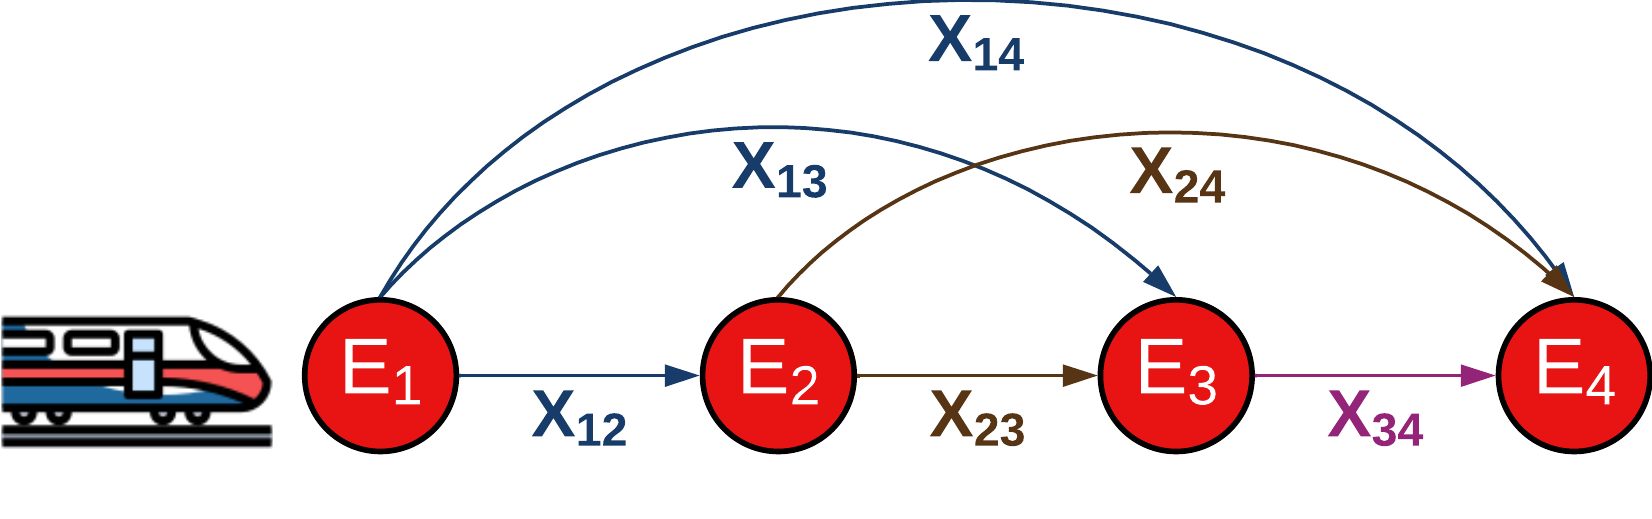
\includegraphics[scale=0.18]{img/repre_ini1.png}
		\caption{Versão gráfica simples}
		% Fonte:~\cite{khaksar2013genetic}}
		\label{fig: fig1}
	\end{center}
\end{figure}


\section{Primeira modelagem matemática}\label{sec:modelo1}

Agora, para a primeira proposta de modelagem, temos o seguinte

\noindent $x_{ij}$: Quantidade de assentos que serão seguradas no trecho com origem em $i$ e destino em $j$, onde $j>i$ (variavel de decisão). \\
\noindent $A_i$: Quantidade de assentos vagos na estação $i$. \\
\noindent $P_{ij}$: Preço da passagem no trajeto com origem em $i$ e destino em $j$. \\
\noindent $Q$: Capacidade física do trem.

Dado o exposto, a função objetivo será maximizar o lucro para cada possível venda em cada trajeto $i,j$, matematicamente seria:

$FO: max \quad x_{12}P_{12} + x_{13}P_{13} + x_{14}P_{14} + x_{23}P_{23} + x_{24}P_{24} + x_{34}P_{34}$

s.a.

Estação 1: $x_{12} + x_{13} + x_{14} \leq A_1 \quad onde \quad A_1 = Q $ \\
\indent Estação 2: $x_{23} + x_{24}  \leq  A_2 \quad onde \quad A_2 = A_1 - (x_{12} + x_{13} + x_{14}) + x_{12} $ \\
\indent Estação 3: $x_{34} \leq A_3 \quad onde \quad A_3 = A_2 - (x_{23} + x_{24}) + x_{13} + x_{23} $

Note que as restrições são aplicadas para cada uma das três primeiras estações, E1, E2 e E3, já que são as estações que têm pelo menos um destino, e a última estação, E4, é excluída, pois não possui nenhum destino.

Cada uma das restrições leva em consideração o fluxo de pessoas que sairão e entrarão no trem. Levando isso em conta, é necessário calcular a disponibilidade do trem para cada estação. Considere uma solução viável para o modelo, conforme mostrado na figura \ref{fig: fig2}, com uma capacidade total de 100 assentos para um trem.

\begin{figure}[!ht]
	\begin{center}
		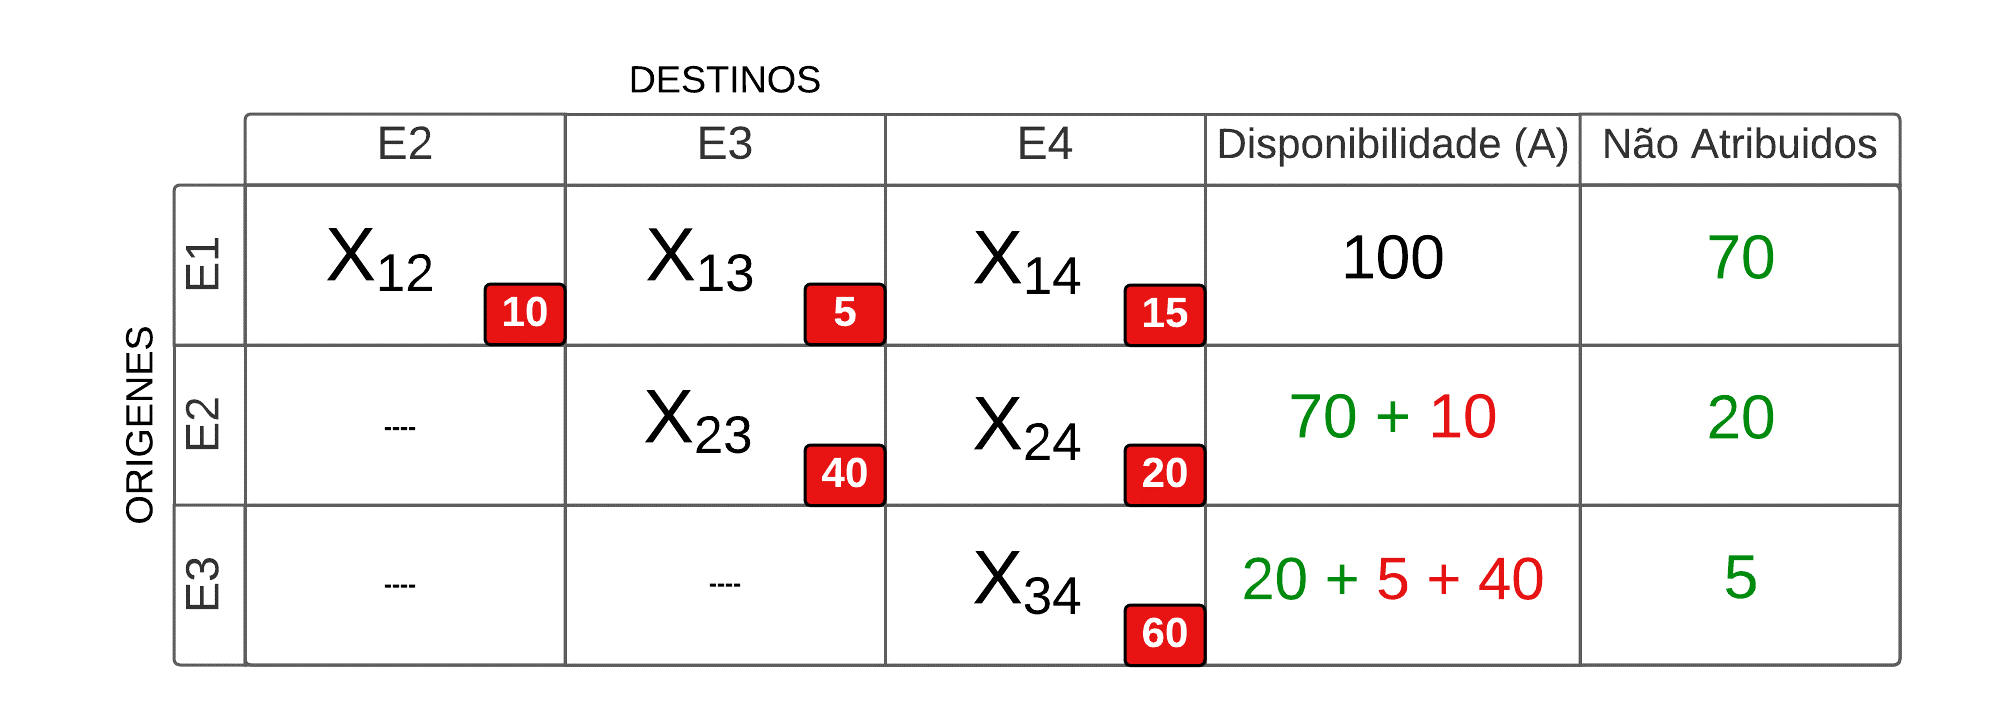
\includegraphics[scale=0.4]{img/fig2.png}
		\caption{Solução factível para o problema simplificado}
		% Fonte:~\cite{khaksar2013genetic}}
		\label{fig: fig2}
	\end{center}
\end{figure}

Note que, para a restrição da estação 1, o trem está com todos os assentos vazios, ou seja, \(A_1=100\), e que a soma das variáveis seria \(x_{12} + x_{13} + x_{14} = 10 + 5 + 15 = 30\). Portanto, teríamos \(30 \leq 100\), ou seja, foram disponibilizados para venda 30 assentos dos 100 que o trem possui. Nesse sentido, no momento da partida do trem da estação 1, haveria 70 assentos vazios ou disponíveis para venda em estações posteriores.

Agora, para a estação 2, teríamos \(A_2 = 100 - 30 + 10 = 70 + 10 = 80\). Já era conhecido que havia 70 assentos disponíveis vindos da estação 1, mas também é preciso levar em conta que os assentos com destino à estação 2 também ficarão disponíveis da estação 2 em diante, para este caso \(x_{12} = 10\). Portanto, para a estação 2, teríamos 80 assentos vazios para disponibilizar, ou seja, \(60 \leq 80\). Analogamente, o mesmo raciocínio seria aplicado para a estação 3, ou seja, teríamos a soma de todos os assentos que chegaram à estação 3, \(x_{13} = 5\) e \(x_{23} = 40\), assim teríamos \(A_3 = 80 - 60 + 5 + 40 = 20 + 5 + 40 = 65\), e no final teríamos \(60 \leq 65\).

Além da lógica anterior, assume-se que há um trem, com vários vagões ou cabines, que viajará de uma estação $E_1$ até uma estação $E_n$ (onde $n$ é a última estação onde o trem chegará). Esse trem terá um itinerário que conterá o nome do trem, a estação de origem, a estação de destino, a data e hora de partida e de chegada. Além disso, haverá uma lista de preços (para o mesmo tipo de assento) a ser disponibilizada para venda. Cada um dos preços da lista será chamado de classe de controle ou control class. Os bilhetes serão disponibilizados para venda antes da partida do trem, e o tempo entre a disponibilização e a referida partida será chamado de horizonte de reserva. Esse horizonte será dividido em vários períodos, que podem ter diferentes temporalidades. Por exemplo, pode haver períodos em dias, semanas, meses, etc., e combinações entre eles. Cada um desses períodos será chamado de check point.

Cada relação possível entre uma estação e outra será denominada origem-destino ou trecho. Será dito que uma origem-destino é adjacente se, e somente se, não houver estações intermediárias entre elas; caso contrário, serão não adjacentes. Por exemplo, na figura \ref{fig: fig1}, os trechos adjacentes seriam: E1-E2, E2-E3, E3-E4, e os trechos não adjacentes seriam: E1-E3, E1-E4 e E2-E4. Além disso, observe que os trechos não adjacentes podem conter outros trechos, tanto adjacentes quanto não adjacentes. Por exemplo, o trecho E1-E4 da figura \ref{fig: fig1} contém os trechos adjacentes E1-E2, E2-E3, e contém os trechos não adjacentes E1-E3 e E2-E4.

Vejamos agora o modelo proposto completo:

\begin{table}[H]
	\centering
	\small
	\begin{tabular}{p{2cm} p{9.5cm} p{3.2cm}}
		\toprule
		\textbf{Definição} & \textbf{Descrição}                                                                                                                                            & \textbf{Domínio}                             \\ \midrule
		\multicolumn{3}{l}{\textbf{Conjuntos}}                                                                                                                                                                                          \\ \midrule
		$O$                & Conjunto de Estações de origem                                                                                                                          &                                              \\
		$D$                & Conjunto de Estações de Destino                                                                                                                          &                                              \\
		$OD$               & Conjunto de Trechos com itinerario                                                                                                                          &                                              \\
		$NAD$              & Conjunto de Trechos que NÃO são Adjacentes e que tem itinerario                                                                                             &                                              \\
		$BRI_{(o,d)}$      & Conjunto de Trechos contidos dentro de cada trecho $(o,d)$ NÃO Adjacente                                                                                    &                                              \\
		$V$                & Conjunto de Cabines do trem                                                                                                                                 &                                              \\
		$T$                & Conjunto de Check-Points (Períodos)                                                                                                                         &                                              \\ 
		$K_v$              & É o conjunto de classes de controle para cada vagão $v$. Por exemplo, suponha que há duas cabines $z$ e $p$, e cada cabine contém três classes de controle $c_1, c_2, c_3$, então a representação seria $K_z:\{c_1,c_2,c_3\}$ e $K_p:\{c_1,c_2,c_3\}$. Além disso, considere que os elementos de cada $K_v$ são ordenados, onde sempre se cumpre que a classe de menor indice é a classe mais costosa, ou seja $c_1>c_2>c_3$.                                                                                                        &                                              \\ \midrule
		\multicolumn{3}{l}{\textbf{Parâmetros}}                                                                                                                                                                                         \\ \midrule
		$n$                & Quantidade de Estações                                                                                                                                                 &                                              \\
		$Q$                & Capacidade física do trem                                                                                                                                          &                                              \\
		$P_{ijvk}$         & Preços  das passagem no Trecho $(i,j)$, Cabine $v$ e Classe de Control $k$                                                                                  & $(i,j) \in OD,v \in V, k \in K_v$            \\
		$d_{ijvkt}$        & Demanda no Trecho $(i,j)$, Cabine $v$ e Classe de Control $k$                                                                                 & $(i,j) \in OD,v \in V, k \in K_v, t \in T$   \\ \midrule
		\multicolumn{3}{l}{\textbf{Variáveis de decisão}}                                                                                                                                                                               \\ \midrule
		$X_{ijvkt}$        & Quantidade de passagem atribuídos no trecho $(i,j)$, cabine $v$ e com classe de control $k$ no período $t$                                                  & $(i,j) \in OD, v \in V, k \in K_v, t \in T$  \\
		$Y_{ijvkt}$        & Quantidade de passagem autorizados no trecho $(i,j)$, cabine $v$ e com classe de control $k$ no período $t$                                                 & $(i,j) \in OD, v \in V, k \in K_v, t \in T$  \\
		$BNA_{ijvkt}$      & É uma variavel binaria que toma o valor de 1 quando $Y_{ijvkt} \neq 0$ e toma  valor de 0 caso contrario, aplica-se apenas a trechos que não são adjacentes & $(i,j) \in NAD, v \in V, k \in K_v, t \in T$ \\\midrule
		\multicolumn{3}{l}{\textbf{Variável auxiliar}}                                                                                                                                                                               \\ \midrule
		$A_{i}$            & Armazena a quantidade de assentos vazios disponíveis para venda em cada estação de origem durante todo o horizonte de reserva. Cabe esclarecer que esta não é uma variável de decisão, pois esta variável apenas armazena um cálculo com base na capacidade física do trem e nas variáveis de decisão de atribuições                                                                                                     & $i \in O$                                    \\
		\bottomrule
	\end{tabular}
	\caption{Notação matemática}
	\label{tab: m1_definicao}
\end{table}

\begin{align}
	& Max \quad Z = \sum_{(i,j)\in OD} \sum_{v\in V} \sum_{k\in K_v} \sum_{t\in T} P_{ijvk} X_{ijvkt}                                                                                                                \label{eq: m1_fo}                          \\
	& \text{s.a.}  \notag                                                                                                                                                                                                                                       \\
	& A_{i} = A_{i-1} - \sum_{(i,j) \in OD/j \geq i} \sum_{v\in V} \sum_{k\in K_v}\sum_{t\in T}X_{i-1,j,v,k,t} + \sum_{(i,j) \in OD/j<i}\sum_{v\in V} \sum_{k\in K_v}\sum_{t\in T}X_{jivkt}, \quad \forall i \in O  \label{eq: m1_disponi}                     \\
	& \sum_{(i,j) \in OD}\sum_{v\in V} \sum_{k\in K_v}\sum_{t\in T} X_{ijvkt} \leq A_{i} , \quad \forall i \in O /i<j, i < n                                                                                        \label{eq: m1_cap_assig}                   \\
	& Y_{ijvkt} \geq Y_{i,j,v,k+1,t},  \quad \forall (i,j) \in OD / i < j, v \in V, k \in K_v / k < \lVert K_v \rVert , t \in T                                                                                                                     \label{eq: m1_jerar_class}                 \\   % P_{ijvk} \geq P_{i,j,v,k+1}
	& X_{ijvkt} \leq d_{ijvkt},  \quad \forall (i,j) \in OD / i < j  ,v \in V, k \in K_v, t\in T                                                                                                                                                  \label{eq: m1_assig_menor_dem}             \\
	& \sum_{(i,j) \in OD}\sum_{v\in V}\sum_{t\in T} Y_{i,j,v,k,t} \leq Q, \quad  k = min\{K_v\}, \forall i \in O                                                                                                  \label{eq: m1_cap_autho_1er_class}         \\
	& Y_{i,j,v,k,t} \geq  X_{i,j,v,k,t},  \quad k = max\{K_v\}, \forall(i,j) \in OD ,v \in V, t \in T                                                                                                                                     \label{eq: m1_autho_mayor_assig_1er_class} \\
	& Y_{i,j,v,k,t} \geq  X_{i,j,v,k,t} + Y_{i,j,v,k + 1,t} , \forall(i,j) \in OD, v \in V, k \in K_v / k < \lVert K_v \rVert , t \in T                                                                                                            \label{eq: m1_autho_mayor_assig_mas_autho} \\
	& BNA_{o,d,v,k,t} \leq Y_{o,d,v,k,t} \leq BNA_{o,d,v,k,t} Q, \quad  \forall (o,d)\in NAD, v \in V, k \in K_v, t \in T                                                                                                                \label{eq: m1_activ_bin_autho}            \\
	& BNA_{o,d,v,k,t} \leq Y_{i,j,v,k,t} \leq BNA_{o,d,v,k,t} Q, \quad  \forall (o,d)\in NAD, (i,j) \in BRI_{(o,d)}, v \in V, k \in K_v, t \in T                                                                                            \label{eq: m1_autho_igualar_trecho_maior}  \\
	& X_{0,j,v,k,t} = 0,     \quad \forall j \in D, k \in K_v, t \in T                                                                                                                                                                     \label{eq: m1_ini_assig}                   \\
	& A_{0} = Q                                                                                                                                                                                                      \label{eq: m1_ini_disponi}                 \\
	& X_{ijvkt} \in \mathbb{Z}^+                                                                                                                                                                                     \label{eq: m1_dom_assig}                   \\
	& Y_{ijvkt} \in \mathbb{Z}^+                                                                                                                                                                                     \label{eq: m1_dom_autho}                   \\
	& A_{j} \in \mathbb{Z}^+                                                                                                                                                                                         \label{eq: m1_dom_disponi}                 \\
	& BNA_{ijvkt} \in \{0,1\}                                                                                                                                                                                        \label{eq: m1_dom_bin_nadja}
\end{align}
% \begin{align}      
% 	& Y_{i,j,v,k,t} \geq  X_{i,j,v,k,t},  \quad k = max\{K_v\}, \forall(i,j),v,t                                                                                                                                     \label{eq: m1_autho_mayor_assig_1er_class} \\
% 	& Y_{i,j,v,k,t} \geq  X_{i,j,v,k,t} + Y_{i,j,v,k + 1,t} , \forall(i,j),v, k, t / k < \lVert K_v\rVert                                                                                                            \label{eq: m1_autho_mayor_assig_mas_autho} \\
% 	& BNA_{o,d,v,k,t} \leq Y_{o,d,v,k,t} \leq BNA_{o,d,v,k,t} Q, \quad  \forall (o,d)\in NAD, v, k, t                                                                                                                \label{eq: m1_activ_bin_autho}             \\
% 	& BNA_{o,d,v,k,t} \leq Y_{i,j,v,k,t} \leq BNA_{o,d,v,k,t} Q, \quad  \forall (o,d)\in NAD, (i,j) \in BRI_{(o,d)}, v,k,t                                                                                           \label{eq: m1_autho_igualar_trecho_maior}  \\
% 	& X_{0,j,v,k,t} = 0,     \quad \forall j,k,t                                                                                                                                                                     \label{eq: m1_ini_assig}                   \\
% 	& A_{0} = Q                                                                                                                                                                                                      \label{eq: m1_ini_disponi}                 \\
% 	& X_{ijvkt} \in \mathbb{Z}^+                                                                                                                                                                                     \label{eq: m1_dom_assig}                   \\
% 	& Y_{ijvkt} \in \mathbb{Z}^+                                                                                                                                                                                     \label{eq: m1_dom_autho}                   \\
% 	& A_{j} \in \mathbb{Z}^+                                                                                                                                                                                         \label{eq: m1_dom_disponi}                 \\
% 	& BNA_{ijvkt} \in \{0,1\}                                                                                                                                                                                        \label{eq: m1_dom_bin_nadja}
% \end{align}


Na equação \ref{eq: m1_fo}, a qual representa a função objetivo, temos a soma do produto entre a quantidade de assentos atribuídos a cada trajeto de origem e destino para a classe comercial em cada período e cada vagão, multiplicada pelo preço correspondente para cada trajeto e classe. Observe que queremos maximizar os ingressos em função dos assentos que estão atribuídos, que é o mais próximo que se tem da realidade em função da demanda conhecida.

A restrição \ref{eq: m1_disponi} é utilizada para calcular a disponibilidade de assentos de cada estação de origem, em cada período de tempo para cada classe em cada vagão e é a generalização do exemplo simplificado para calcular a variável auxiliar $A_i$.

A restrição \ref{eq: m1_cap_assig} garante que todas as autorizações habilitadas a partir de cada estação de origem para cada período e cada classe de cada vagão não excedam a disponibilidade da sua estação de origem correspondente (a disponibilidades é calculada na restrição \ref{eq: m1_disponi}).

A restrição \ref{eq: m1_jerar_class} é uma restrição de hierarquia e garante que as quantidades de autorizações para as classes de maior preço sejam sempre maiores do que as quantidades de autorizações de menor preço em cada vagão, em cada trecho, e em  cada período do horizonte de reserva.

A restrição \ref{eq: m1_assig_menor_dem} garante que a quantidade de atribuições não ultrapasse a demanda para cada trecho de cada classe em cada vagoen e em cada período no horizonte de reserva.

A restrição \ref{eq: m1_cap_autho_1er_class} garanta que a soma de autorizações da classe mais costosa de cada vagão, de cada estação de origem, de tudos os periodos, não ultrapase a capacidade do trem, note que apenas estamos considerando a classe mais cara devido à natureza cumulativa das variáveis de autorização é por isso que o valor de k é o mínimo das classes de cada vagão, pois a ordem do nome das classes é crescente mas o seu valor é decrescente. Para melhor compreensão, suponhamos uma solução para um problema de dois vagões $V_1$ e $V_2$, 3 classes para $V_1$ e 3 classes para $V_2$, 5 estações,  10 trechos, um período e uma capacidade física do trem de 700 cadeiras, conforme mostra a figura \ref{fig: autorization}.

\begin{figure}[!ht]
	\begin{center}
		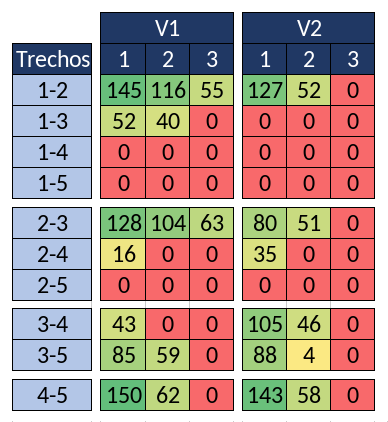
\includegraphics[scale=0.40]{img/exemplo1.png}
		\caption{Solução factível para a variavel de desição Autorização}
		% Fonte:~\cite{khaksar2013genetic}}
		\label{fig: autorization}
	\end{center}
\end{figure}

Observe que os nomes das classes são números ordenados de forma crescente [1, 2, 3] também o valor da classe 1 é mais caro que o valor da classe 2 e este é maior que o valor da classe 3. Além disso, a soma que não ultrapassará a capacidade do trem é a soma das classes 1 de cada vagão de cada estação de origem. Por exemplo, para a estação 3 seria $43 + 85$ para $V_1$ trecho 3-4 e 3-5, mais, $105 + 88$ para $V_2$ nos mesmos trechos, ou seja $43 + 85 + 105 + 88 = 321 \leq 700$  


Até ao momento foi referido que a variável $Y$ tem um carácter cumulativo e são as restrições \ref{eq: m1_autho_mayor_assig_1er_class} e \ref{eq: m1_autho_mayor_assig_mas_autho} que controlam este comportamento. A restrição \ref{eq: m1_autho_mayor_assig_1er_class} é um caso particular da restrição \ref{eq: m1_autho_mayor_assig_mas_autho}, aplicada apenas à última classe, ou classe mais barata atribuída para cada vagão ($k=max\{K_v\}$), e garante que a soma de todos os períodos, de cada estação de origem da classe mais barata da variável "autorização" é maior ou igual à variável de decisão "segurada" nas mesmas condições. Por outro lado, a restrição \ref{eq: m1_autho_mayor_assig_mas_autho} garante que cada classe autorizada seja sempre maior ou igual à classe autorizada imediatamente menor, mais a quantidade segurada da mesma classe, isto para cada período, cada trecho e cada classe diferente da classe mais barata. Para melhor compreensão, assuma as mesmas suposições que foram feitas na restrição \ref{eq: m1_cap_autho_1er_class} %com a diferença que agora as tabelas representam uma solução factivel para a soma de n períodos e não um único período.


\begin{figure}[h!]
	\centering
	\begin{subfigure}[b]{0.35\linewidth}
		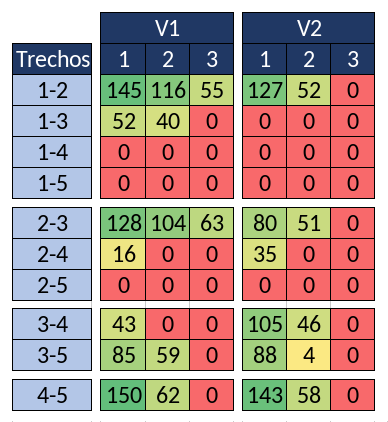
\includegraphics[width=\linewidth]{img/exemplo1.png}
		\caption{Autorização [Variavel $Y$]}
		\label{fig:auto_assig_a}
	\end{subfigure}\hspace{5mm}
	\begin{subfigure}[b]{0.35\linewidth}
		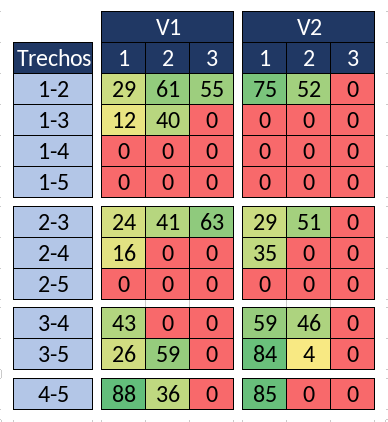
\includegraphics[width=\linewidth]{img/exemplo2.png}
		\caption{Atribução [Variavel $X$]}
		\label{fig:auto_assig_b}
	\end{subfigure}
	\caption{Solução factível para as variaveis de desição Autorização e Atribução}
	\label{fig:auto_assig}
\end{figure}

Observe a linha correspondente ao trecho 1-2 do vagão $V_2$ na tabela \ref{fig:auto_assig_b}, veja que a classe segurada mais barata foi a classe 2 com valor de 52, por este motivo na tabela \ref{fig:auto_assig_a} na mesma posição o valor deverá ser igual ou maior que 52, que neste caso é o mesmo valor; Agora observe para o mesmo trecho para o vagão $V_1$ classe 3 em ambas as tabelas acontece a mesma coisa, esse comportamento é garantido pela restrição \ref{eq: m1_autho_mayor_assig_1er_class}. Agora não vamos olhar para a classe mais barata, vamos olhar para qualquer outra, por exemplo, para o mesmo trecho veja a classe 1 do vagão $V_1$ da tabela \ref{fig:auto_assig_b} com valor 29, se quiséssemos saber o valor correspondente na tabela \ref{fig:auto_assig_a} deveríamos adicionar a classe imediata menor (à direita) da classe 1 na tabela \ref{fig:auto_assig_a}, neste caso seria a classe 2 com valor 116, e some o valor da classe 1 da tabela \ref{fig:auto_assig_b}, que já sabemos que é 29, assim, o valor buscado será maior ou igual a $116+29 = 145$, como visto em tabela \ref{fig:auto_assig_a}, lembre-se que nessa posição o valor mínimo será o calculado, mas poderá assumir um valor superior. Esta última situação é controlada pela restrição \ref{eq: m1_autho_mayor_assig_mas_autho}.

Suponha que você tem um trecho não adjacente E1-E3, e que esse trecho contém outros trechos E1-E2 e E2-E3. Para esta situação, a classe mais barata ativada no trecho E1-E3 deverá ser a classe mais barata ativada nos trechos E1-E2 e E2-E3. Isso é feito com o objetivo de que as combinações dos preços dos bilhetes por trechos não sejam mais econômicos do que o preço de um bilhete direto. Para alcançar isso, é criada uma variável binária para cada trecho não adjacente ($BNA$), que será ativada, ou tomará o valor de 1, quando as atribuições $"Y"$ (ou assentos a serem disponibilizados para venda) de uma classe desse trecho, de um vagão e de um período, forem diferentes de zero e tomará o valor de zero caso contrário. Esse comportamento será controlado pela restrição \ref{eq: m1_activ_bin_autho}.

Uma vez calculados os valores para $BNA$ dos trechos não adjacentes, a restrição \ref{eq: m1_autho_igualar_trecho_maior} fará com que as classes de controle de todos os trechos contidos em cada trecho não adjacente sejam $0$ ou, no mínimo $1$. Assim, quando a classe de controle do trecho não adjacente assumir um valor de $BNA = 0$, essa classe será $0$ para os trechos contidos. Por outro lado, se a classe de controle do trecho não adjacente assumir o valor de $BNA = 1$, então essa classe tomará, no mínimo, o valor de $1$ para todos os trechos contidos.

Para um melhor entendimento, suponha um trem com 1 vagão que passa por 3 estações, $E_1$, $E_2$ e $E_3$, e tem um horizonte de reserva de um único período. Sob esta situação, o trecho não adjacente seria $"E_1-E_3"$ e os trechos contidos seriam $"E_1-E_2"$ e $"E_2-E_3"$. Agora imagine que cada trecho tem 6 classes diferentes ($c_1, c_2, c_3, c_4, c_5, c_6$), onde o preço  de  $c_1 \geq c_2 \geq c_3 \geq c_4 \geq c_5 \geq c_6$, e que as autorizações (variavel $Y$) tomam os valores mostrados na tabela \ref{fig: exemplo_sip}:

\begin{figure}[!ht]
	\begin{center}
		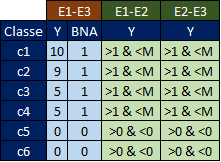
\includegraphics[scale=0.8]{img/tab_trechos_maiores.png}
		\caption{Exemplo simplificado do funcionamento da restrição \ref{eq: m1_autho_igualar_trecho_maior}}
		% Fonte:~\cite{khaksar2013genetic}}
		\label{fig: exemplo_sip}
	\end{center}
\end{figure}

Para o trecho $"E_1-E_3"$, note que quando $Y \neq 0$, $BNA = 1$ e quando $Y = 0$, $BNA = 0$ (controlado pela restrição \ref{eq: m1_activ_bin_autho}). Agora observe que, quando $ BNA = 1$ para uma certa classe, os trechos $E_1-E_2$ e $E_2-E_3$ assumem valores entre 1 e um número suficientemente grande ($1 \le Y \leq M$), o que indica que os assentos a serem disponibilizados para essa classe nesses trechos não podem ser zero. Por outro lado, quando $BNA = 0$, os trechos menores devem zerar a classe correspondente com ($0 \leq Y \leq 0$), ou seja, não se deve disponibilizar assentos com essa classe (controlado pela restrição \ref{eq: m1_autho_igualar_trecho_maior}). Deve-se esclarecer que as classe de controle dos trechos contidos, apenas imitam o comportamento da classe não adjacente correspondente, e não os valores que esta assume.

As restrições de \ref{eq: m1_ini_assig} e \ref{eq: m1_ini_disponi} são usadas para inicializar a restrição \ref{eq: m1_disponi} quando \(i = 1\). E as restrições de \ref{eq: m1_dom_assig} a \ref{eq: m1_dom_bin_nadja} representam o domínio das variáveis.

\section{Segunda modelagem matemática}\label{sec:modelo2}

Vamos considerar novamente uma versão simplificada do problema. Na verdade, para esta modelagem, serão levadas em conta as mesmas variáveis do primeiro modelo, exceto a variável de disponibilidade \(A\), conforme mostrado a seguir:

\noindent $x_{ij}$: Quantidade de assentos que será disponibilizada para venda no trecho com origem em $i$ e destino em $j$, onde $j>i$ \\
\noindent $P_{ij}$: Preço da passagem no trajeto com origem em $i$ e destino em $j$ \\
\noindent $Q$: Capacidade do trem

\noindent Assim, a função objetivo e as restrições são como segue:

$FO: max \quad x_{12}P_{12} + x_{13}P_{13} + x_{14}P_{14} + x_{23}P_{23} + x_{24}P_{24} + x_{34}P_{34}$

s.a.

\noindent{\it Restrições para estações de origem}

Estação 1: $x_{12} + x_{13} + x_{14} \leq Q $ \\
\indent Estação 2: $x_{23} + x_{24}  \leq  Q $ \\
\indent Estação 3: $x_{34} \leq Q $

\noindent{\it Restrições para estações de destino}

Estação 2: $x_{12} \leq Q $ \\
\indent Estação 3: $x_{13} + x_{23}  \leq  Q $ \\
\indent Estação 4: $x_{14} + x_{24} + x_{34} \leq Q $

Observe que esta formulação é baseada nos modelos de transporte, onde as estações de origem seriam os depósitos e estão restritas por sua capacidade (capacidade do trem), e as estações de destino seriam os destinos e estão restritas, neste caso, pela mesma capacidade do trem e não pela demanda de cada destino.

Esta formulação garante que sempre será disponibilizada, no máximo, a capacidade do trem tanto para cada saída quanto para cada chegada do trem. Imagine uma solução viável como a mostrada na figura \ref{fig: fig2}.

\begin{figure}[h]
	\begin{center}
		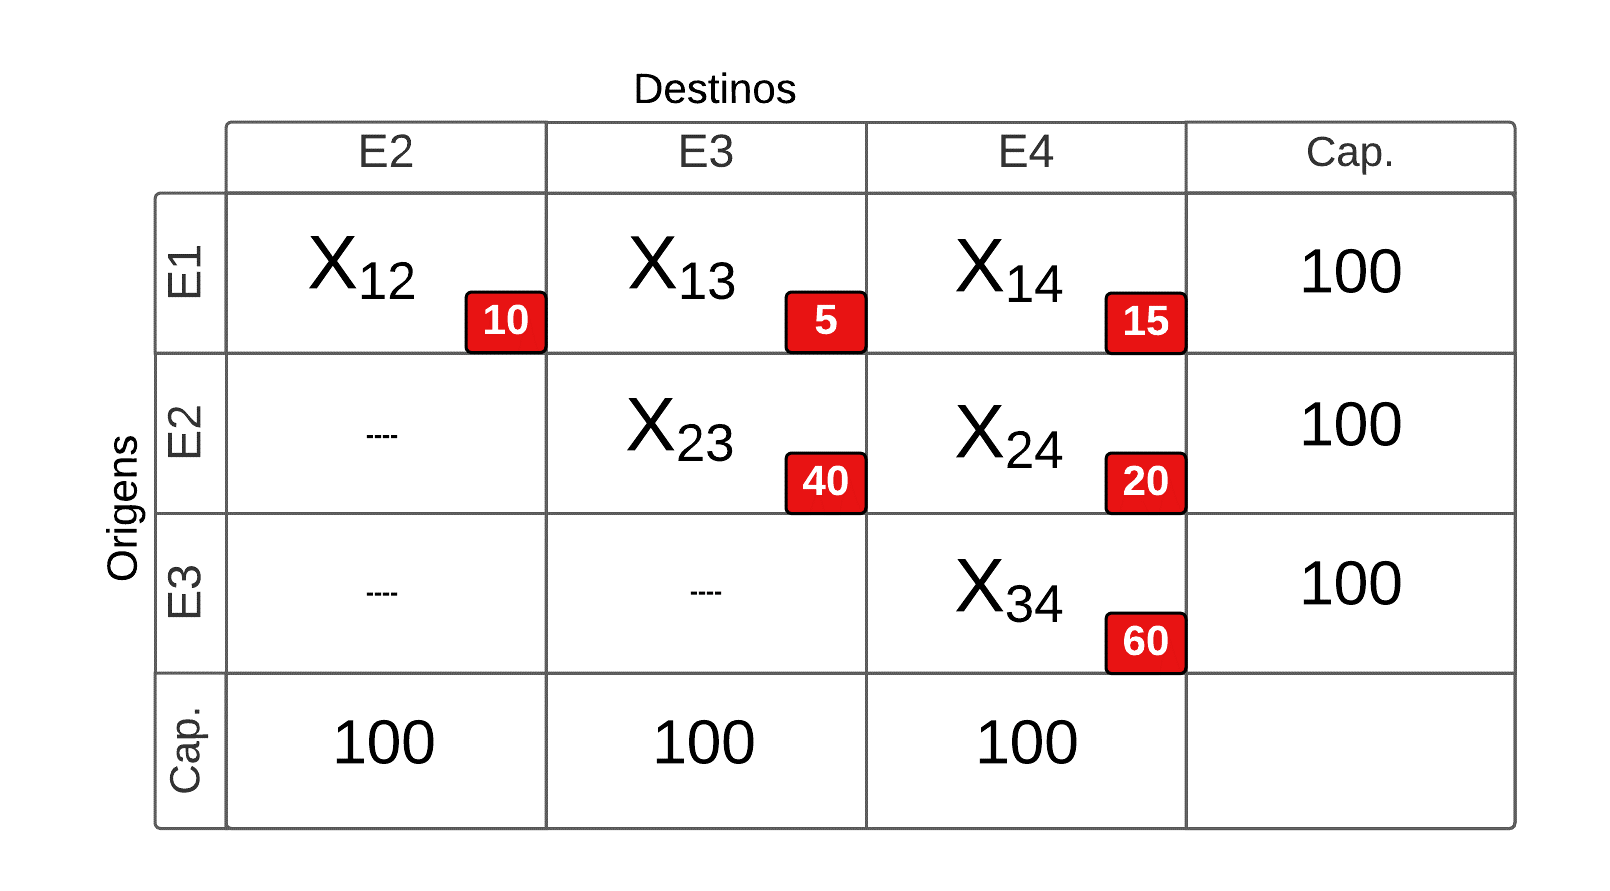
\includegraphics[scale=0.4]{img/fig3.png}
		\caption{Solução factível para o problema simplificado}
		% Fonte:~\cite{khaksar2013genetic}}
		\label{fig: fig3}
	\end{center}
\end{figure}

Observe que os valores das variáveis são os mesmos que foram mostrados na figura \ref{fig: fig3}. E ainda todas as restrições, tanto por linha quanto por coluna (por origens e por destinos), continuam sendo atendidas.

\begin{table}[h]
	\centering
	\small
	\begin{tabular}{p{2cm} p{9.5cm} p{3.2cm}}
		\toprule
		\textbf{Definição} & \textbf{Notação}                                                                                                                                            & \textbf{Domínio}                             \\ \midrule
		\multicolumn{3}{l}{\textbf{Conjuntos}}                                                                                                                                                                                          \\ \midrule
		$OD$               & Conjunto de Trechos com itinerario                                                                                                                          &                                              \\
		$NAD$              & Conjunto de Trechos que NÃO são Adjacentes e que tem itinerario                                                                                             &                                              \\
		$BRI_{(o,d)}$      & Conjunto de Trechos contidos dentro de cada trecho $(o,d)$ NÃO Adjacente                                                                                    &                                              \\
		$V$                & Conjunto de Cabines do trem                                                                                                                                 &                                              \\
		$K_v$              & Conjunto de Classes de Control de cada cabine em $V$                                                                                                        &                                              \\
		$T$                & Conjunto de Check-Points (Períodos)                                                                                                                         &                                              \\ \midrule
		\multicolumn{3}{l}{\textbf{Parâmetros}}                                                                                                                                                                                         \\ \midrule
		$Q$                & Capacidade do trem                                                                                                                                          &                                              \\
		$P_{ijvk}$         & Preços  das passagem no Trecho $(i,j)$, Cabine $v$ e Classe de Control $k$                                                                                  & $(i,j) \in OD,v \in V, k \in K_v$            \\
		$D_{ijvkt}$        & Demanda  das passagem no Trecho $(i,j)$, Cabine $v$ e Classe de Control $k$                                                                                 & $(i,j) \in OD,v \in V, k \in K_v, t \in T$   \\ \midrule
		\multicolumn{3}{l}{\textbf{Variáveis de decisão}}                                                                                                                                                                               \\ \midrule
		$X_{ijvkt}$        & Quantidade de passagem atribuídos no trecho $(i,j)$, cabine $v$ e com classe de control $k$ no período $t$                                                  & $(i,j) \in OD, v \in V, k \in K_v, t \in T$  \\
		$Y_{ijvkt}$        & Quantidade de passagem autorizados no trecho $(i,j)$, cabine $v$ e com classe de control $k$ no período $t$                                                 & $(i,j) \in OD, v \in V, k \in K_v, t \in T$  \\
		$BNA_{ijvkt}$      & É uma variavel binaria que toma o valor de 1 quando $Y_{ijvkt} \neq 0$ e toma  valor de 0 caso contrario, aplica-se apenas a trechos que não são adjacentes & $(i,j) \in NAD, v \in V, k \in K_v, t \in T$ \\
		\bottomrule
	\end{tabular}
	\caption{Notação matemática}
	\label{tab: m2_definicao}
\end{table}
\begin{align}
	 & Max \quad Z = \sum_{(i,j)\in OD} \sum_{v\in V} \sum_{k\in K_v} \sum_{t\in T} P_{ijvk} X_{ijvkt}                                 \label{eq: m2_fo}                          \\
	 & \text{s.a.}  \notag                                                                                                                                                        \\
	 & \sum_{(i,j)\in OD}\sum_{v\in V}\sum_{k\in K_v}\sum_{t\in T}X_{ijvkt} \leq Q , \quad \forall j / j>1, i<j                        \label{eq: m2_cap_assig_destino}           \\
	 & \sum_{(i,j)\in OD}\sum_{v\in V}\sum_{k\in K_v}\sum_{t\in T}X_{ijvkt} \leq Q , \quad \forall i / i<n, j>i                        \label{eq: m2_cap_assig_origem}            \\
	 & Y_{ijvkt} \geq Y_{i,j,v,k+1,t},  \quad \forall (i,j),v,k,t / i < j, k < \lVert K_v \rVert,  P_{ijvk} \geq P_{i,j,v,k+1}         \label{eq: m2_jerar_class}                 \\
	 & X_{ijvkt} \leq D_{ijvkt},  \quad \forall (i,j),v,k,t/ i < j                                                                     \label{eq: m2_assig_menor_dem}             \\
	 & \sum_{(i,j) \in OD}\sum_{v\in V}\sum_{t\in T} Y_{i,j,v,k,t} \leq Q, \quad  k = min\{K_v\}, \forall i \in OD                     \label{eq: m2_cap_autho_1er_class}         \\
	 & Y_{i,j,v,k,t} \geq  X_{i,j,v,k,t},  \quad k = max\{K_v\}, \forall(i,j),v,t                                                      \label{eq: m2_autho_mayor_assig_1er_class} \\
	 & Y_{i,j,v,k,t} \geq  X_{i,j,v,k,t} + Y_{i,j,v,k + 1,t} , \forall(i,j),v, k, t / k < \lVert K_v\rVert                             \label{eq: m2_autho_mayor_assig_mas_autho} %\\
	%  & BNA_{o,d,v,k,t} \leq Y_{o,d,v,k,t} \leq BNA_{o,d,v,k,t} Q, \quad  \forall (o,d)\in NAD, v, k, t                                 \label{eq: m2_activ_bin_autho}             \\
	%  & BNA_{o,d,v,k,t} \leq Y_{i,j,v,k,t} \leq BNA_{o,d,v,k,t} Q, \quad  \forall (o,d)\in NAD, (i,j) \in BRI_{(o,d)}, v,k,t            \label{eq: m2_autho_igualar_trecho_maior}  \\
	%  & X_{ijvkt} \in \mathbb{Z}^+                                                                                                      \label{eq: m2_dom_assig}                  %\\
\end{align}
\begin{align}
	& BNA_{o,d,v,k,t} \leq Y_{o,d,v,k,t} \leq BNA_{o,d,v,k,t} Q, \quad  \forall (o,d)\in NAD, v, k, t                                 \label{eq: m2_activ_bin_autho}             \\
	& BNA_{o,d,v,k,t} \leq Y_{i,j,v,k,t} \leq BNA_{o,d,v,k,t} Q, \quad  \forall (o,d)\in NAD, (i,j) \in BRI_{(o,d)}, v,k,t            \label{eq: m2_autho_igualar_trecho_maior}  \\
	& X_{ijvkt} \in \mathbb{Z}^+                                                                                                      \label{eq: m2_dom_assig}                   \\
	& Y_{ijvkt} \in \mathbb{Z}^+                                                                                                      \label{eq: m2_dom_autho}                   \\
	& BNA_{ijvkt} \in \{0,1\}                                                                                                         \label{eq: m2_dom_bin_nadja}
\end{align}

Como já foi mencionado, nesta formulação modificamos as restrições que controlam as variáveis asseguradas X, ou seja, mudamos as restrições 1 e 2 do primeiro modelo e eliminamos a variável de decisão Ai.

% \end{adjustwidth}
%Note que, na definição, não temos mais a variável de decisão de disponibilidade \(A_i\). Neste caso, a equação \ref{eq: m2_fo} representa a função objetivo que esta tentando maximizar a soma do produto entre as quantidades seguradas e os preços das mesmas, ou seja, estamos maximizando a receita em função das quantidades dos assentos que estão assegurados.

%A restrição \ref{eq: m2_cap_assig_destino} garante que a quantidade total de assentos autorizados para cada destino seja a quantidade máxima de assentos do trem para todas as classes e todos os períodos.
%A restrição \ref{eq: m2_cap_assig_origem} garante que a quantidade de assentos autorizados para cada origem seja no máximo a capacidade do trem para todas as classes e todos os períodos.
%As restrições de \ref{eq: m2_cap_autho_1er_class} a \ref{eq: m2_dom_autho} representam o mesmo que o primeiro modelo já exposto.\\

Para este caso, as restrições \ref{eq: m2_cap_assig_destino} e \ref{eq: m2_cap_assig_origem} representam a generalização do problema simplificado, onde a primeira garante que a quantidade de assentos autorizados para venda não viole a capacidade do trem ao chegar a cada estação de destino; e a segunda garante que a quantidade de assentos autorizados respeite a capacidade do trem no momento de sair de cada estação de origem. O restante das restrições foi explicado na formulação 1.
% \input{Contribuicoes}
% %\input{Metodos-de-resolucao-propostos}
% type:ignore

\chapter{Resultados Computacionais}

% \section{Modelos Matemáticos}
% Embora três modelos matemáticos tenham sido propostos — a formulação independente e as formulações comportamentais —, ao resolver as instâncias decidiu-se inicialmente testar os modelos sem as restrições de fulfillment nem as restrições de skiplagging. Em seguida, cada modelo foi testado separadamente com cada grupo de restrições. Por fim, ambos os modelos foram avaliados considerando os dois conjuntos de restrições simultaneamente. Essa abordagem foi adotada para observar como a solução evoluía ou se comportava ao incluir cada tipo de restrição no modelo. Dito isso, a seguir são apresentados os modelos com suas respectivas descrições.
% \vspace{0.5cm}

% \begin{small}
% 	\begin{longtable}{p{5.4cm} p{10.4cm}}
% 		\hline
% 		\textbf{Tipo de Modelo}            & \textbf{Descrição}                                                                                                                       \\ \hline
% 		BaseModel                          & Modelo base independente sem as restrições de Fulfillments nem as restrições de Skiplagging.                                             \\ \hline
% 		BaseModelFulfillments              & Modelo base independente com as restrições de Fulfillments.                                                                              \\ \hline
% 		BaseModelSkiplagging               & Modelo base independente com as restrições de Skiplagging.                                                                               \\ \hline
% 		BaseModelFull                      & Modelo independente completo com os dois conjuntos de restrições.                                                                        \\ \hline
% 		HierarBehavioralModel              & Modelo base comportamental com ajuste de demanda do tipo hierarquia, sem as restrições de Fulfillments nem as restrições de Skiplagging. \\ \hline
% 		HierarBehavioralModelFulfillments  & Modelo base comportamental com ajuste de demanda do tipo hierarquia, com as restrições de Fulfillments.                                  \\ \hline
% 		HierarBehavioralModelSkiplagging   & Modelo base comportamental com ajuste de demanda do tipo hierarquia, com as restrições de Skiplagging.                                   \\ \hline
% 		HierarBehavioralModelFull          & Modelo comportamental completo com ajuste de demanda do tipo hierarquia, com os dois conjuntos de restrições.                            \\ \hline
% 		PercentBehavioralModel             & Modelo base comportamental com ajuste de demanda do tipo proporção, sem as restrições de Fulfillments nem as restrições de Skiplagging.  \\ \hline
% 		PercentBehavioralModelFulfillments & Modelo base comportamental com ajuste de demanda do tipo proporção, com as restrições de Fulfillments.                                   \\ \hline
% 		PercentBehavioralModelSkiplagging  & Modelo base comportamental com ajuste de demanda do tipo proporção, com as restrições de Skiplagging.                                    \\ \hline
% 		PercentBehavioralModelFull         & Modelo comportamental completo com ajuste de demanda do tipo proporção, com os dois conjuntos de restrições.                             \\ \hline
% 		\caption{Descrição dos modelos matemáticos propostos}
% 		\label{tab:modelos}
% 	\end{longtable}
% \end{small}


% \section{Instâncias}

% Para verificar as características dos modelos propostos, foram utilizadas 10 instâncias reais fornecidas pela empresa canadense Expetrio. As características de cada uma dessas instâncias estão apresentadas na Tabela \ref{tab:instancias}.

% \begin{table}[H]
% 	\centering
% 	\begin{tabular}{ccccccc}
% 		\toprule
% 		\textbf{Instância}                                                  &
% 		\textbf{\begin{tabular}[c]{@{}c@{}}Nome \\ Trem\end{tabular}}       &
% 		\textbf{\begin{tabular}[c]{@{}c@{}}Capacidade \\ Trem\end{tabular}} &
% 		\textbf{Data Partida}                                               &
% 		\textbf{\# Trechos}                                                 &
% 		\textbf{\# Períodos}                                                &
% 		\textbf{\# Classes}                                                                                          \\
% 		\midrule
% 		Inst1                                                          & 68 & 561 & 2023-11-21 & 256 & 120 & 15 \\
% 		Inst2                                                          & 13 & 637 & 2023-11-26 & 252 & 146 & 15 \\
% 		Inst3                                                          & 71 & 563 & 2023-10-13 & 250 & 105 & 16 \\
% 		Inst4                                                          & 71 & 561 & 2023-11-21 & 241 & 124 & 15 \\\midrule
% 		Inst5                                                          & 8  & 561 & 2022-12-04 & 152 & 116 & 17 \\
% 		Inst6                                                          & 40 & 565 & 2023-11-21 & 149 & 68  & 16 \\
% 		Inst7                                                          & 74 & 491 & 2023-07-25 & 136 & 70  & 16 \\\midrule
% 		Inst8                                                          & 72 & 493 & 2023-10-25 & 100 & 85  & 16 \\
% 		Inst9                                                          & 45 & 563 & 2023-03-16 & 90  & 73  & 16 \\
% 		Inst10                                                         & 15 & 493 & 2023-08-07 & 50  & 60  & 12 \\
% 		\bottomrule
% 	\end{tabular}
% 	\caption{Resumo das instâncias utilizadas no experimento}
% 	\label{tab:instancias}
% \end{table}

% A coluna "\# Trechos" \, representa a quantidade de trechos que a viagem do trem possui em cada instância. A coluna "\# Períodos" \, indica a quantidade de períodos considerados na programação desse trajeto dentro do seu horizonte de reserva. Por fim, a coluna "\# Classes" \, mostra o número máximo de classes disponíveis para cada viagem de cada trem; Observe que, para cada trecho, podem estar disponíveis todas as classes indicadas na coluna correspondente ou uma quantidade menor.

% Por outro lado, afirmamos que as instâncias compreendidas entre a Instância1 e a Instância4 são classificadas como grandes, as instâncias entre a Instância5 e a Instância7 como médias, e as demais como pequenas.

\section{Experimentos Computacionais}
Para resolver as instâncias utilizando os modelos matemáticos propostos, foi empregado um computador da marca Dell, modelo Precision 3660, equipado com o sistema operacional Windows 11 Pro de 64 bits, processador 13th Gen Intel(R) Core(TM) i7-13700 2.10 GHz baseado em arquitetura x64, e memória RAM de 16GB. Além disso, utilizou-se o Python como linguagem de programação na versão 3.10.14, e o solver Gurobi na versão 11.0.3.

Em primeiro lugar, apresentam-se os resultados de cada instância após serem resolvidas por meio de cada um dos modelos propostos. Essa organização busca evidenciar de forma clara e comparativa o desempenho dos modelos em diferentes cenários, destacando as principais diferenças e similaridades nas soluções obtidas para cada instância.

Observe que a primeira coluna indica o nome do modelo utilizado. A segunda coluna, "\textit{T. Criação Modelo (seg.)}", exibe o tempo, em segundos, que o solver levou para construir o modelo. A terceira coluna, "\textit{T. Solução (seg.)}", mostra o tempo necessário para que o solver resolvesse o modelo. A sétima coluna, "\textit{Z Relaxado}", apresenta a relaxação linear do problema no nó raiz. Já a oitava coluna, "\textit{Z\*}", indica o valor ótimo da função objetivo (máximo lucro encontrado). Por fim, a nona coluna, "\textit{$ \Delta Z (\%)$}", mostra a diferença percentual entre a solução relaxada e a solução ótima.

\begin{table}[H]
    \centering
    \resizebox{\textwidth}{!}{%
        \begin{tabular}{lccccccccc}
            \hline
            \textbf{Modelo} &
            \textbf{\begin{tabular}[c]{@{}c@{}}T. Criação \\ Modelo (seg.)\end{tabular}} &
            \textbf{\begin{tabular}[c]{@{}c@{}}T. Solução \\ (seg.)\end{tabular}} &
            \textbf{\begin{tabular}[c]{@{}c@{}}N° Nós \\ Explorados\end{tabular}} &
            \textbf{\begin{tabular}[c]{@{}c@{}}N° \\ Iterações\end{tabular}} &
            \textbf{\begin{tabular}[c]{@{}c@{}}N° \\ Soluções\end{tabular}} &
            \textbf{\begin{tabular}[c]{@{}c@{}}Z \\ Relaxado\end{tabular}} &
            \textbf{Z*} &
            \textbf{\begin{tabular}[c]{@{}c@{}}$\Delta$ Z \\ (\%)\end{tabular}} \\ \hline
            BaseModel & 2,30 & 0,07 & 1 & 0 & 1 & 170.485 & 170.485 & 0,00 \\ 
            BaseModelFulfillments & 3,97 & 0,07 & 1 & 0 & 1 & 170.485 & 170.485 & 0,00 \\ 
            BaseModelSkiplagging & 6,06 & 0,06 & 1 & 0 & 1 & 133.237 & 133.237 & 0,00 \\ 
            BaseModelFull & 6,43 & 0,05 & 1 & 0 & 1 & 51.410 & 51.410 & 0,00 \\ 
            HierarBehavioralModel & 3,17 & 0,07 & 1 & 0 & 1 & 170.455 & 170.455 & 0,00 \\ 
            HierarBehavioralModelFulfillments & 4,87 & 0,08 & 1 & 0 & 1 & 170.455 & 170.455 & 0,00 \\ 
            HierarBehavioralModelSkiplagging & 7,09 & 0,08 & 1 & 2 & 2 & 132.928 & 132.928 & 0,00 \\ 
            HierarBehavioralModelFull & 7,48 & 0,05 & 1 & 0 & 1 & 51.336 & 51.336 & 0,00 \\ 
            PercentBehavioralModel & 3,14 & 0,07 & 1 & 0 & 1 & 166.345 & 166.345 & 0,00 \\ 
            PercentBehavioralModelFulfillments & 4,90 & 0,08 & 1 & 0 & 1 & 170.455 & 170.455 & 0,00 \\ 
            PercentBehavioralModelSkiplagging & 7,07 & 0,06 & 1 & 2 & 2 & 132.928 & 132.928 & 0,00 \\ 
            PercentBehavioralModelFull & 7,47 & 0,05 & 1 & 0 & 1 & 51.336 & 51.336 & 0,00 \\ \hline
        \end{tabular}%
    }
    \caption{Resultados para a Instância1}
    \label{tab:resultado_instancia1}
\end{table}

\begin{table}[H]
    \centering
    \resizebox{\textwidth}{!}{%
        \begin{tabular}{lccccccccc}
            \hline
            \textbf{Modelo} &
            \textbf{\begin{tabular}[c]{@{}c@{}}T. Criação \\ Modelo (seg.)\end{tabular}} &
            \textbf{\begin{tabular}[c]{@{}c@{}}T. Solução \\(seg.)\end{tabular}} &
            \textbf{\begin{tabular}[c]{@{}c@{}}N° Nós \\Explorado\end{tabular}} &
            \textbf{\begin{tabular}[c]{@{}c@{}}N° \\Iterações\end{tabular}} &
            \textbf{\begin{tabular}[c]{@{}c@{}}N° \\Soluções\end{tabular}} &
            \textbf{\begin{tabular}[c]{@{}c@{}}Z \\Relaxado\end{tabular}} &
            \textbf{Z*} &
            \textbf{\begin{tabular}[c]{@{}c@{}}$\Delta$ Z \\(\%)\end{tabular}} \\ \hline
            BaseModel & 2,90 & 0,08 & 1 & 0 & 1 & 314.883,03 & 314.883,03 & 0,00 \\ 
            BaseModelFulfillments & 5,22 & 0,08 & 1 & 0 & 1 & 314.883,03 & 314.883,03 & 0,00 \\ 
            BaseModelSkiplagging & 7,47 & 0,07 & 1 & 0 & 1 & 303.634,13 & 303.634,13 & 0,00 \\ 
            BaseModelFull & 8,00 & 0,07 & 1 & 0 & 1 & 203.208,98 & 203.208,98 & 0,00 \\ 
            HierarBehavioralModel & 3,98 & 0,07 & 1 & 0 & 1 & 314.599,53 & 314.599,53 & 0,00 \\ 
            HierarBehavioralModelFulfillments & 6,38 & 0,10 & 1 & 0 & 3 & 314.599,53 & 314.599,53 & 0,00 \\ 
            HierarBehavioralModelSkiplagging & 8,58 & 0,06 & 1 & 0 & 1 & 303.375,63 & 303.375,63 & 0,00 \\ 
            HierarBehavioralModelFull & 9,11 & 0,07 & 1 & 0 & 1 & 203.276,98 & 203.276,98 & 0,00 \\ 
            PercentBehavioralModel & 3,98 & 0,07 & 1 & 0 & 1 & 313.547,03 & 313.547,03 & 0,00 \\ 
            PercentBehavioralModelFulfillments & 6,35 & 0,10 & 1 & 0 & 3 & 314.599,53 & 314.599,53 & 0,00 \\ 
            PercentBehavioralModelSkiplagging & 8,62 & 0,06 & 1 & 0 & 1 & 303.375,63 & 303.375,63 & 0,00 \\ 
            PercentBehavioralModelFull & 9,20 & 0,08 & 1 & 0 & 1 & 203.276,98 & 203.276,98 & 0,00 \\ \hline
        \end{tabular}%
    }
    \caption{Resultados para a Instância2}
    \label{tab:resultado_instancia2}
\end{table}


\begin{table}[H]
    \centering
    \resizebox{\textwidth}{!}{%
        \begin{tabular}{lccccccccc}
            \hline
            \textbf{Modelo} &
            \textbf{\begin{tabular}[c]{@{}c@{}}T. Criação \\ Modelo (seg.)\end{tabular}} &
            \textbf{\begin{tabular}[c]{@{}c@{}}T. Solução \\(seg.)\end{tabular}} &
            \textbf{\begin{tabular}[c]{@{}c@{}}N° Nós \\Explorado\end{tabular}} &
            \textbf{\begin{tabular}[c]{@{}c@{}}N° \\Iterações\end{tabular}} &
            \textbf{\begin{tabular}[c]{@{}c@{}}N° \\Soluções\end{tabular}} &
            \textbf{\begin{tabular}[c]{@{}c@{}}Z \\Relaxado\end{tabular}} &
            \textbf{Z*} &
            \textbf{\begin{tabular}[c]{@{}c@{}}$\Delta$ Z \\(\%)\end{tabular}} \\ \hline
            BaseModel & 2,25 & 0,05 & 1 & 33 & 2 & 140.788,61 & 140.788,61 & 0,00 \\ 
            BaseModelFulfillments & 3,75 & 0,08 & 1 & 377 & 2 & 140.788,61 & 140.788,61 & 0,00 \\ 
            BaseModelSkiplagging & 18,62 & 0,07 & 1 & 25 & 2 & 95.625,49 & 95.625,49 & 0,00 \\ 
            BaseModelFull & 19,15 & 0,05 & 1 & 0 & 1 & 37.214,03 & 37.214,03 & 0,00 \\ 
            \textbf{HierarBehavioralModel} &\textbf{3,01}&\textbf{0,08}& \textbf{1} & \textbf{97}&\textbf{6} & \textbf{140.179,10} & \textbf{140.167,27}& \textbf{0,01} \\ 
            \textbf{HierarBehavioralModelFulfillments} & \textbf{4,67} &\textbf{0,12} &\textbf{1} & \textbf{571}& \textbf{10} & \textbf{140.086,16}& \textbf{140.077,33} &\textbf{0,01} \\ 
            HierarBehavioralModelSkiplagging & 19,87 & 0,06 & 1 & 55 & 3 & 95.101,49 & 95.101,49 & 0,00 \\ 
            HierarBehavioralModelFull & 20,08 & 0,05 & 1 & 4 & 4 & 37.183,03 & 37.183,03 & 0,00 \\ 
            PercentBehavioralModel & 3,02 & 0,05 & 1 & 35 & 2 & 136.487,26 & 136.487,26 & 0,00 \\ 
            \textbf{PercentBehavioralModelFulfillments} & \textbf{4,67} & \textbf{0,12} & \textbf{1} &\textbf{571} &\textbf{10} & \textbf{140.086,16} &\textbf{140.077,33 }&\textbf{0,01} \\ 
            PercentBehavioralModelSkiplagging & 20,09 & 0,05 & 1 & 55 & 3 & 95.101,49 & 95.101,49 & 0,00 \\ 
            PercentBehavioralModelFull & 20,43 & 0,05 & 1 & 4 & 4 & 37.183,03 & 37.183,03 & 0,00 \\ \hline
        \end{tabular}%
    }
    \caption{Resultados para a Instância3}
    \label{tab:resultado_instancia3}
\end{table}


\begin{table}[H]
    \centering
    \resizebox{\textwidth}{!}{%
        \begin{tabular}{lccccccccc}
            \hline
            \textbf{Modelo} &
            \textbf{\begin{tabular}[c]{@{}c@{}}T. Criação \\ Modelo (seg.)\end{tabular}} &
            \textbf{\begin{tabular}[c]{@{}c@{}}T. Solução \\(seg.)\end{tabular}} &
            \textbf{\begin{tabular}[c]{@{}c@{}}N° Nós \\Explorado\end{tabular}} &
            \textbf{\begin{tabular}[c]{@{}c@{}}N° \\Iterações\end{tabular}} &
            \textbf{\begin{tabular}[c]{@{}c@{}}N° \\Soluções\end{tabular}} &
            \textbf{\begin{tabular}[c]{@{}c@{}}Z \\Relaxado\end{tabular}} &
            \textbf{Z*} &
            \textbf{\begin{tabular}[c]{@{}c@{}}$\Delta$ Z \\(\%)\end{tabular}} \\ \hline
            BaseModel & 2,20 & 0,05 & 1 & 0 & 1 & 166.118,29 & 166.118,29 & 0,00 \\
            BaseModelFulfillments & 3,70 & 0,08 & 1 & 0 & 1 & 166.118,29 & 166.118,29 & 0,00 \\
            BaseModelSkiplagging & 4,65 & 0,07 & 1 & 0 & 1 & 130.810,41 & 130.810,41 & 0,00 \\
            BaseModelFull & 4,95 & 0,04 & 1 & 0 & 1 & 40.602,31 & 40.602,31 & 0,00 \\
            HierarBehavioralModel & 3,02 & 0,05 & 1 & 0 & 1 & 165.869,29 & 165.869,29 & 0,00 \\
            HierarBehavioralModelFulfillments & 4,48 & 0,07 & 1 & 0 & 1 & 165.869,29 & 165.869,29 & 0,00 \\
            HierarBehavioralModelSkiplagging & 5,50 & 0,05 & 1 & 0 & 2 & 129.740,41 & 129.740,41 & 0,00 \\
            HierarBehavioralModelFull & 5,84 & 0,04 & 1 & 0 & 1 & 40.718,31 & 40.718,31 & 0,00 \\
            PercentBehavioralModel & 3,07 & 0,05 & 1 & 0 & 1 & 162.681,09 & 162.681,09 & 0,00 \\
            PercentBehavioralModelFulfillments & 4,52 & 0,08 & 1 & 0 & 1 & 165.869,29 & 165.869,29 & 0,00 \\
            PercentBehavioralModelSkiplagging & 5,47 & 0,07 & 1 & 0 & 2 & 129.740,41 & 129.740,41 & 0,00 \\
            PercentBehavioralModelFull & 5,73 & 0,05 & 1 & 0 & 1 & 40.718,31 & 40.718,31 & 0,00 \\ \hline
        \end{tabular}%
    }
    \caption{Resultados para a Instância4}
    \label{tab:resultado_instancia4}
\end{table}


\begin{table}[H]
    \centering
    \resizebox{\textwidth}{!}{%
        \begin{tabular}{lccccccccc}
            \hline
            \textbf{Modelo} &
            \textbf{\begin{tabular}[c]{@{}c@{}}T. Criação \\ Modelo (seg.)\end{tabular}} &
            \textbf{\begin{tabular}[c]{@{}c@{}}T. Solução \\(seg.)\end{tabular}} &
            \textbf{\begin{tabular}[c]{@{}c@{}}N° Nós \\Explorado\end{tabular}} &
            \textbf{\begin{tabular}[c]{@{}c@{}}N° \\Iterações\end{tabular}} &
            \textbf{\begin{tabular}[c]{@{}c@{}}N° \\Soluções\end{tabular}} &
            \textbf{\begin{tabular}[c]{@{}c@{}}Z \\Relaxado\end{tabular}} &
            \textbf{Z*} &
            \textbf{\begin{tabular}[c]{@{}c@{}}$\Delta$ Z \\(\%)\end{tabular}} \\ \hline
            BaseModel & 2,20 & 0,05 & 1 & 29  & 3 & 127.371,39 & 127.371,39 & 0,00 \\
            BaseModelFulfillments & 3,07 & 0,07 & 1 & 143 & 4 & 127.371,39 & 127.371,39 & 0,00 \\
            BaseModelSkiplagging & 3,05 & 0,07 & 1 & 0   & 1 & 95.816,84  & 95.816,84  & 0,00 \\
            BaseModelFull & 3,24 & 0,05 & 1 & 0   & 1 & 28.647,69 & 28.647,69 & 0,00 \\
            \textbf{HierarBehavioralModel} & \textbf{2,72} & \textbf{0,05} & \textbf{1} & \textbf{53}  & \textbf{4} & \textbf{127.020,39} & \textbf{127.010,39} & \textbf{0,01} \\
            \textbf{HierarBehavioralModelFulfillments} & \textbf{3,58} & \textbf{0,07} & \textbf{1} & \textbf{170} & \textbf{4} & \textbf{127.020,39} & \textbf{127.010,39} & \textbf{0,01} \\
            HierarBehavioralModelSkiplagging & 3,58 & 0,07 & 1 & 0   & 1 & 95.403,84  & 95.403,84  & 0,00 \\
            HierarBehavioralModelFull & 3,87 & 0,06 & 1 & 0   & 1 & 28.460,69 & 28.460,69 & 0,00 \\
            PercentBehavioralModel & 2,68 & 0,07 & 1 & 34  & 3 & 124.593,69 & 124.593,69 & 0,00 \\
            \textbf{PercentBehavioralModelFulfillments} & \textbf{3,67} & \textbf{0,08} & \textbf{1} & \textbf{170} & \textbf{4} & \textbf{127.020,39} & \textbf{127.010,39} & \textbf{0,01} \\
            PercentBehavioralModelSkiplagging & 3,62 & 0,05 & 1 & 0   & 1 & 95.403,84  & 95.403,84  & 0,00 \\
            PercentBehavioralModelFull & 3,85 & 0,05 & 1 & 0   & 1 & 28.460,69 & 28.460,69 & 0,00 \\ \hline
        \end{tabular}%
    }
    \caption{Resultados para a Instância5}
    \label{tab:resultado_instancia5}
\end{table}


\begin{table}[H]
    \centering
    \resizebox{\textwidth}{!}{%
        \begin{tabular}{lccccccccc}
            \hline
            \textbf{Modelo} &
            \textbf{\begin{tabular}[c]{@{}c@{}}T. Criação \\ Modelo (seg.)\end{tabular}} &
            \textbf{\begin{tabular}[c]{@{}c@{}}T. Solução \\(seg.)\end{tabular}} &
            \textbf{\begin{tabular}[c]{@{}c@{}}N° Nós \\Explorado\end{tabular}} &
            \textbf{\begin{tabular}[c]{@{}c@{}}N° \\Iterações\end{tabular}} &
            \textbf{\begin{tabular}[c]{@{}c@{}}N° \\Soluções\end{tabular}} &
            \textbf{\begin{tabular}[c]{@{}c@{}}Z \\Relaxado\end{tabular}} &
            \textbf{Z*} &
            \textbf{\begin{tabular}[c]{@{}c@{}}$\Delta$ Z \\(\%)\end{tabular}} \\ \hline
            BaseModel & 1,18 & 0,03 & 0 & 0 & 1 & 67.715,07 & 67.715,07 & 0,00 \\
            BaseModelFulfillments & 1,75 & 0,03 & 0 & 0 & 1 & 67.715,07 & 67.715,07 & 0,00 \\
            BaseModelSkiplagging & 1,72 & 0,04 & 0 & 0 & 1 & 51.708,29 & 51.708,29 & 0,00 \\
            BaseModelFull & 1,83 & 0,03 & 0 & 0 & 1 & 24.722,37 & 24.722,37 & 0,00 \\
            HierarBehavioralModel & 1,48 & 0,03 & 0 & 0 & 1 & 67.593,22 & 67.593,22 & 0,00 \\
            HierarBehavioralModelFulfillments & 2,15 & 0,07 & 0 & 0 & 1 & 67.587,22 & 67.587,22 & 0,00 \\
            HierarBehavioralModelSkiplagging & 2,07 & 0,05 & 1 & 0 & 1 & 51.589,44 & 51.589,44 & 0,00 \\
            HierarBehavioralModelFull & 2,27 & 0,03 & 0 & 0 & 1 & 24.714,52 & 24.714,52 & 0,00 \\
            PercentBehavioralModel & 1,48 & 0,03 & 0 & 0 & 1 & 65.256,64 & 65.256,64 & 0,00 \\
            PercentBehavioralModelFulfillments & 2,10 & 0,05 & 0 & 0 & 1 & 67.587,22 & 67.587,22 & 0,00 \\
            PercentBehavioralModelSkiplagging & 2,08 & 0,03 & 1 & 0 & 1 & 51.589,44 & 51.589,44 & 0,00 \\
            PercentBehavioralModelFull & 2,22 & 0,03 & 0 & 0 & 1 & 24.714,52 & 24.714,52 & 0,00 \\ \hline
        \end{tabular}%
    }
    \caption{Resultados para a Instância6}
    \label{tab:resultado_instancia6}
\end{table}


\begin{table}[H]
    \centering
    \resizebox{\textwidth}{!}{%
        \begin{tabular}{lccccccccc}
            \hline
            \textbf{Modelo} &
            \textbf{\begin{tabular}[c]{@{}c@{}}T. Criação \\ Modelo (seg.)\end{tabular}} &
            \textbf{\begin{tabular}[c]{@{}c@{}}T. Solução \\(seg.)\end{tabular}} &
            \textbf{\begin{tabular}[c]{@{}c@{}}N° Nós \\Explorado\end{tabular}} &
            \textbf{\begin{tabular}[c]{@{}c@{}}N° \\Iterações\end{tabular}} &
            \textbf{\begin{tabular}[c]{@{}c@{}}N° \\Soluções\end{tabular}} &
            \textbf{\begin{tabular}[c]{@{}c@{}}Z \\Relaxado\end{tabular}} &
            \textbf{Z*} &
            \textbf{\begin{tabular}[c]{@{}c@{}}$\Delta$ Z \\(\%)\end{tabular}} \\ \hline
            BaseModel & 1,07 & 0,03 & 0 & 0 & 1 & 48.719,71 & 48.719,71 & 0,00 \\
            BaseModelFulfillments & 1,72 & 0,03 & 0 & 0 & 1 & 48.719,71 & 48.719,71 & 0,00 \\
            BaseModelSkiplagging & 1,81 & 0,03 & 0 & 0 & 1 & 20.996,45 & 20.996,45 & 0,00 \\
            BaseModelFull & 1,98 & 0,03 & 0 & 0 & 1 & 9.382,95 & 9.382,95 & 0,00 \\
            HierarBehavioralModel & 1,43 & 0,05 & 1 & 60 & 5 & 47.990,71 & 47.990,71 & 0,00 \\
            HierarBehavioralModelFulfillments & 2,17 & 0,05 & 1 & 227 & 6 & 47.990,71 & 47.990,71 & 0,00 \\
            HierarBehavioralModelSkiplagging & 2,25 & 0,03 & 0 & 0 & 3 & 20.694,45 & 20.694,45 & 0,00 \\
            HierarBehavioralModelFull & 2,37 & 0,05 & 0 & 0 & 1 & 8.663,95 & 8.663,95 & 0,00 \\
            \textbf{PercentBehavioralModel} & \textbf{1,45} & \textbf{0,02} & \textbf{-} & \textbf{-} & \textbf{-} & \textbf{- }& \textbf{Infactível} & \textbf{- }\\
            PercentBehavioralModelFulfillments & 2,17 & 0,05 & 1 & 227 & 6 & 47.990,71 & 47.990,71 & 0,00 \\
            PercentBehavioralModelSkiplagging & 2,25 & 0,03 & 0 & 0 & 3 & 20.694,45 & 20.694,45 & 0,00 \\
            PercentBehavioralModelFull & 2,38 & 0,03 & 0 & 0 & 1 & 8.663,95 & 8.663,95 & 0,00 \\ \hline
        \end{tabular}%
    }
    \caption{Resultados para a Instância7}
    \label{tab:resultado_instancia7}
\end{table}


\begin{table}[H]
    \centering
    \resizebox{\textwidth}{!}{%
        \begin{tabular}{lccccccccc}
            \hline
            \textbf{Modelo} &
            \textbf{\begin{tabular}[c]{@{}c@{}}T. Criação \\ Modelo (seg.)\end{tabular}} &
            \textbf{\begin{tabular}[c]{@{}c@{}}T. Solução \\(seg.)\end{tabular}} &
            \textbf{\begin{tabular}[c]{@{}c@{}}N° Nós \\Explorado\end{tabular}} &
            \textbf{\begin{tabular}[c]{@{}c@{}}N° \\Iterações\end{tabular}} &
            \textbf{\begin{tabular}[c]{@{}c@{}}N° \\Soluções\end{tabular}} &
            \textbf{\begin{tabular}[c]{@{}c@{}}Z \\Relaxado\end{tabular}} &
            \textbf{Z*} &
            \textbf{\begin{tabular}[c]{@{}c@{}}$\Delta$ Z \\(\%)\end{tabular}} \\ \hline
            BaseModel & 0,94 & 0,03 & 0 & 0 & 1 & 53.844,31 & 53.844,31 & 0,00 \\
            BaseModelFulfillments & 1,58 & 0,05 & 0 & 0 & 1 & 53.844,31 & 53.844,31 & 0,00 \\
            BaseModelSkiplagging & 1,57 & 0,04 & 0 & 0 & 1 & 28.675,46 & 28.675,46 & 0,00 \\
            BaseModelFull & 1,70 & 0,03 & 0 & 0 & 1 & 13.985,90 & 13.985,90 & 0,00 \\
            HierarBehavioralModel & 1,32 & 0,03 & 1 & 54 & 5 & 52.091,71 & 52.091,71 & 0,00 \\
            HierarBehavioralModelFulfillments & 1,98 & 0,07 & 1 & 205 & 6 & 52.091,71 & 52.091,71 & 0,00 \\
            HierarBehavioralModelSkiplagging & 1,98 & 0,03 & 0 & 0 & 2 & 28.506,46 & 28.506,46 & 0,00 \\
            HierarBehavioralModelFull & 2,12 & 0,03 & 0 & 0 & 2 & 11.599,90 & 11.599,90 & 0,00 \\
            \textbf{PercentBehavioralModel} & \textbf{1,30} & \textbf{0,02} & \textbf{-} & \textbf{-} & \textbf{-} & \textbf{- }& \textbf{Infactível} & \textbf{- }\\
            PercentBehavioralModelFulfillments & 1,99 & 0,05 & 1 & 205 & 6 & 52.091,71 & 52.091,71 & 0,00 \\
            PercentBehavioralModelSkiplagging & 1,97 & 0,03 & 0 & 0 & 2 & 28.506,46 & 28.506,46 & 0,00 \\
            PercentBehavioralModelFull & 2,12 & 0,03 & 0 & 0 & 2 & 11.599,90 & 11.599,90 & 0,00 \\ \hline
        \end{tabular}%
    }
    \caption{Resultados para a Instância8}
    \label{tab:resultado_instancia8}
\end{table}


\begin{table}[H]
    \centering
    \resizebox{\textwidth}{!}{%
        \begin{tabular}{lccccccccc}
            \hline
            \textbf{Modelo} &
            \textbf{\begin{tabular}[c]{@{}c@{}}T. Criação \\ Model (seg.)\end{tabular}} &
            \textbf{\begin{tabular}[c]{@{}c@{}}T. Solução \\(seg.)\end{tabular}} &
            \textbf{\begin{tabular}[c]{@{}c@{}}N° Nós \\Explorado\end{tabular}} &
            \textbf{\begin{tabular}[c]{@{}c@{}}N° \\Iterações\end{tabular}} &
            \textbf{\begin{tabular}[c]{@{}c@{}}N° \\Soluções\end{tabular}} &
            \textbf{\begin{tabular}[c]{@{}c@{}}Z \\Relaxado\end{tabular}} &
            \textbf{Z*} &
            \textbf{\begin{tabular}[c]{@{}c@{}}$\Delta$ Z \\(\%)\end{tabular}} \\ \hline
            BaseModel & 0,82 & 0,03 & 0 & 0 & 1 & 55.282,08 & 55.282,08 & 0,00 \\
            BaseModelFulfillments & 1,33 & 0,03 & 0 & 0 & 1 & 55.282,08 & 55.282,08 & 0,00 \\
            BaseModelSkiplagging & 1,37 & 0,03 & 0 & 0 & 1 & 33.524,11 & 33.524,11 & 0,00 \\
            BaseModelFull & 1,48 & 0,03 & 0 & 0 & 1 & 9.902,35 & 9.902,35 & 0,00 \\
            HierarBehavioralModel & 1,12 & 0,03 & 0 & 0 & 1 & 55.230,08 & 55.230,08 & 0,00 \\
            HierarBehavioralModelFulfillments & 1,66 & 0,05 & 1 & 13 & 5 & 55.230,08 & 55.230,08 & 0,00 \\
            HierarBehavioralModelSkiplagging & 1,71 & 0,03 & 1 & 3 & 3 & 33.249,11 & 33.249,11 & 0,00 \\
            HierarBehavioralModelFull & 1,85 & 0,03 & 0 & 0 & 1 & 9.726,35 & 9.726,35 & 0,00 \\
            PercentBehavioralModel & 1,12 & 0,03 & 0 & 0 & 1 & 50.834,74 & 50.834,74 & 0,00 \\
            PercentBehavioralModelFulfillments & 1,68 & 0,05 & 1 & 13 & 5 & 55.230,08 & 55.230,08 & 0,00 \\
            PercentBehavioralModelSkiplagging & 1,70 & 0,03 & 1 & 3 & 3 & 33.249,11 & 33.249,11 & 0,00 \\
            PercentBehavioralModelFull & 1,82 & 0,04 & 0 & 0 & 1 & 9.726,35 & 9.726,35 & 0,00 \\ \hline
        \end{tabular}%
    }
    \caption{Resultados para a Instância9}
    \label{tab:resultado_instancia9}
\end{table}


\begin{table}[H]
    \centering
    \resizebox{\textwidth}{!}{%
        \begin{tabular}{lccccccccc}
            \hline
            \textbf{Modelo} &
            \textbf{\begin{tabular}[c]{@{}c@{}}T. Criação \\ Model (seg.)\end{tabular}} &
            \textbf{\begin{tabular}[c]{@{}c@{}}T. Solução \\(seg.)\end{tabular}} &
            \textbf{\begin{tabular}[c]{@{}c@{}}N° Nós \\Explorado\end{tabular}} &
            \textbf{\begin{tabular}[c]{@{}c@{}}N° \\Iterações\end{tabular}} &
            \textbf{\begin{tabular}[c]{@{}c@{}}N° \\Soluções\end{tabular}} &
            \textbf{\begin{tabular}[c]{@{}c@{}}Z \\Relaxado\end{tabular}} &
            \textbf{Z*} &
            \textbf{\begin{tabular}[c]{@{}c@{}}$\Delta$ Z \\(\%)\end{tabular}} \\ \hline
            BaseModel & 0,39 & 0,02 & 0 & 0 & 1 & 21.548,62 & 21.548,62 & 0,00 \\
            BaseModelFulfillments & 0,65 & 0,02 & 0 & 0 & 1 & 21.548,62 & 21.548,62 & 0,00 \\
            BaseModelSkiplagging & 0,64 & 0,00 & 0 & 0 & 1 & 13.102,66 & 13.102,66 & 0,00 \\
            BaseModelFull & 0,70 & 0,01 & 0 & 0 & 1 & 3.637,46 & 3.637,46 & 0,00 \\
            HierarBehavioralModel & 0,56 & 0,02 & 1 & 5 & 3 & 22.112,12 & 22.112,12 & 0,00 \\
            HierarBehavioralModelFulfillments & 0,90 & 0,03 & 1 & 0 & 1 & 22.112,12 & 22.112,12 & 0,00 \\
            HierarBehavioralModelSkiplagging & 0,85 & 0,01 & 1 & 19 & 2 & 13.015,16 & 13.015,16 & 0,00 \\
            HierarBehavioralModelFull & 0,94 & 0,01 & 0 & 0 & 1 & 3.362,96 & 3.362,96 & 0,00 \\
            \textbf{PercentBehavioralModel} & \textbf{0,58} & \textbf{0,00} & \textbf{-} & \textbf{-} & \textbf{-} & \textbf{- }& \textbf{Infactível} & \textbf{- }\\
            PercentBehavioralModelFulfillments & 0,87 & 0,02 & 1 & 0 & 1 & 22.112,12 & 22.112,12 & 0,00 \\
            PercentBehavioralModelSkiplagging & 0,88 & 0,00 & 1 & 19 & 2 & 13.015,16 & 13.015,16 & 0,00 \\
            PercentBehavioralModelFull & 0,95 & 0,02 & 0 & 0 & 1 & 3.362,96 & 3.362,96 & 0,00 \\ \hline
        \end{tabular}%
    }
    \caption{Resultados para a Instância10}
    \label{tab:resultado_instancia10}
\end{table}


\begin{figure}[!ht]
	\begin{center}
		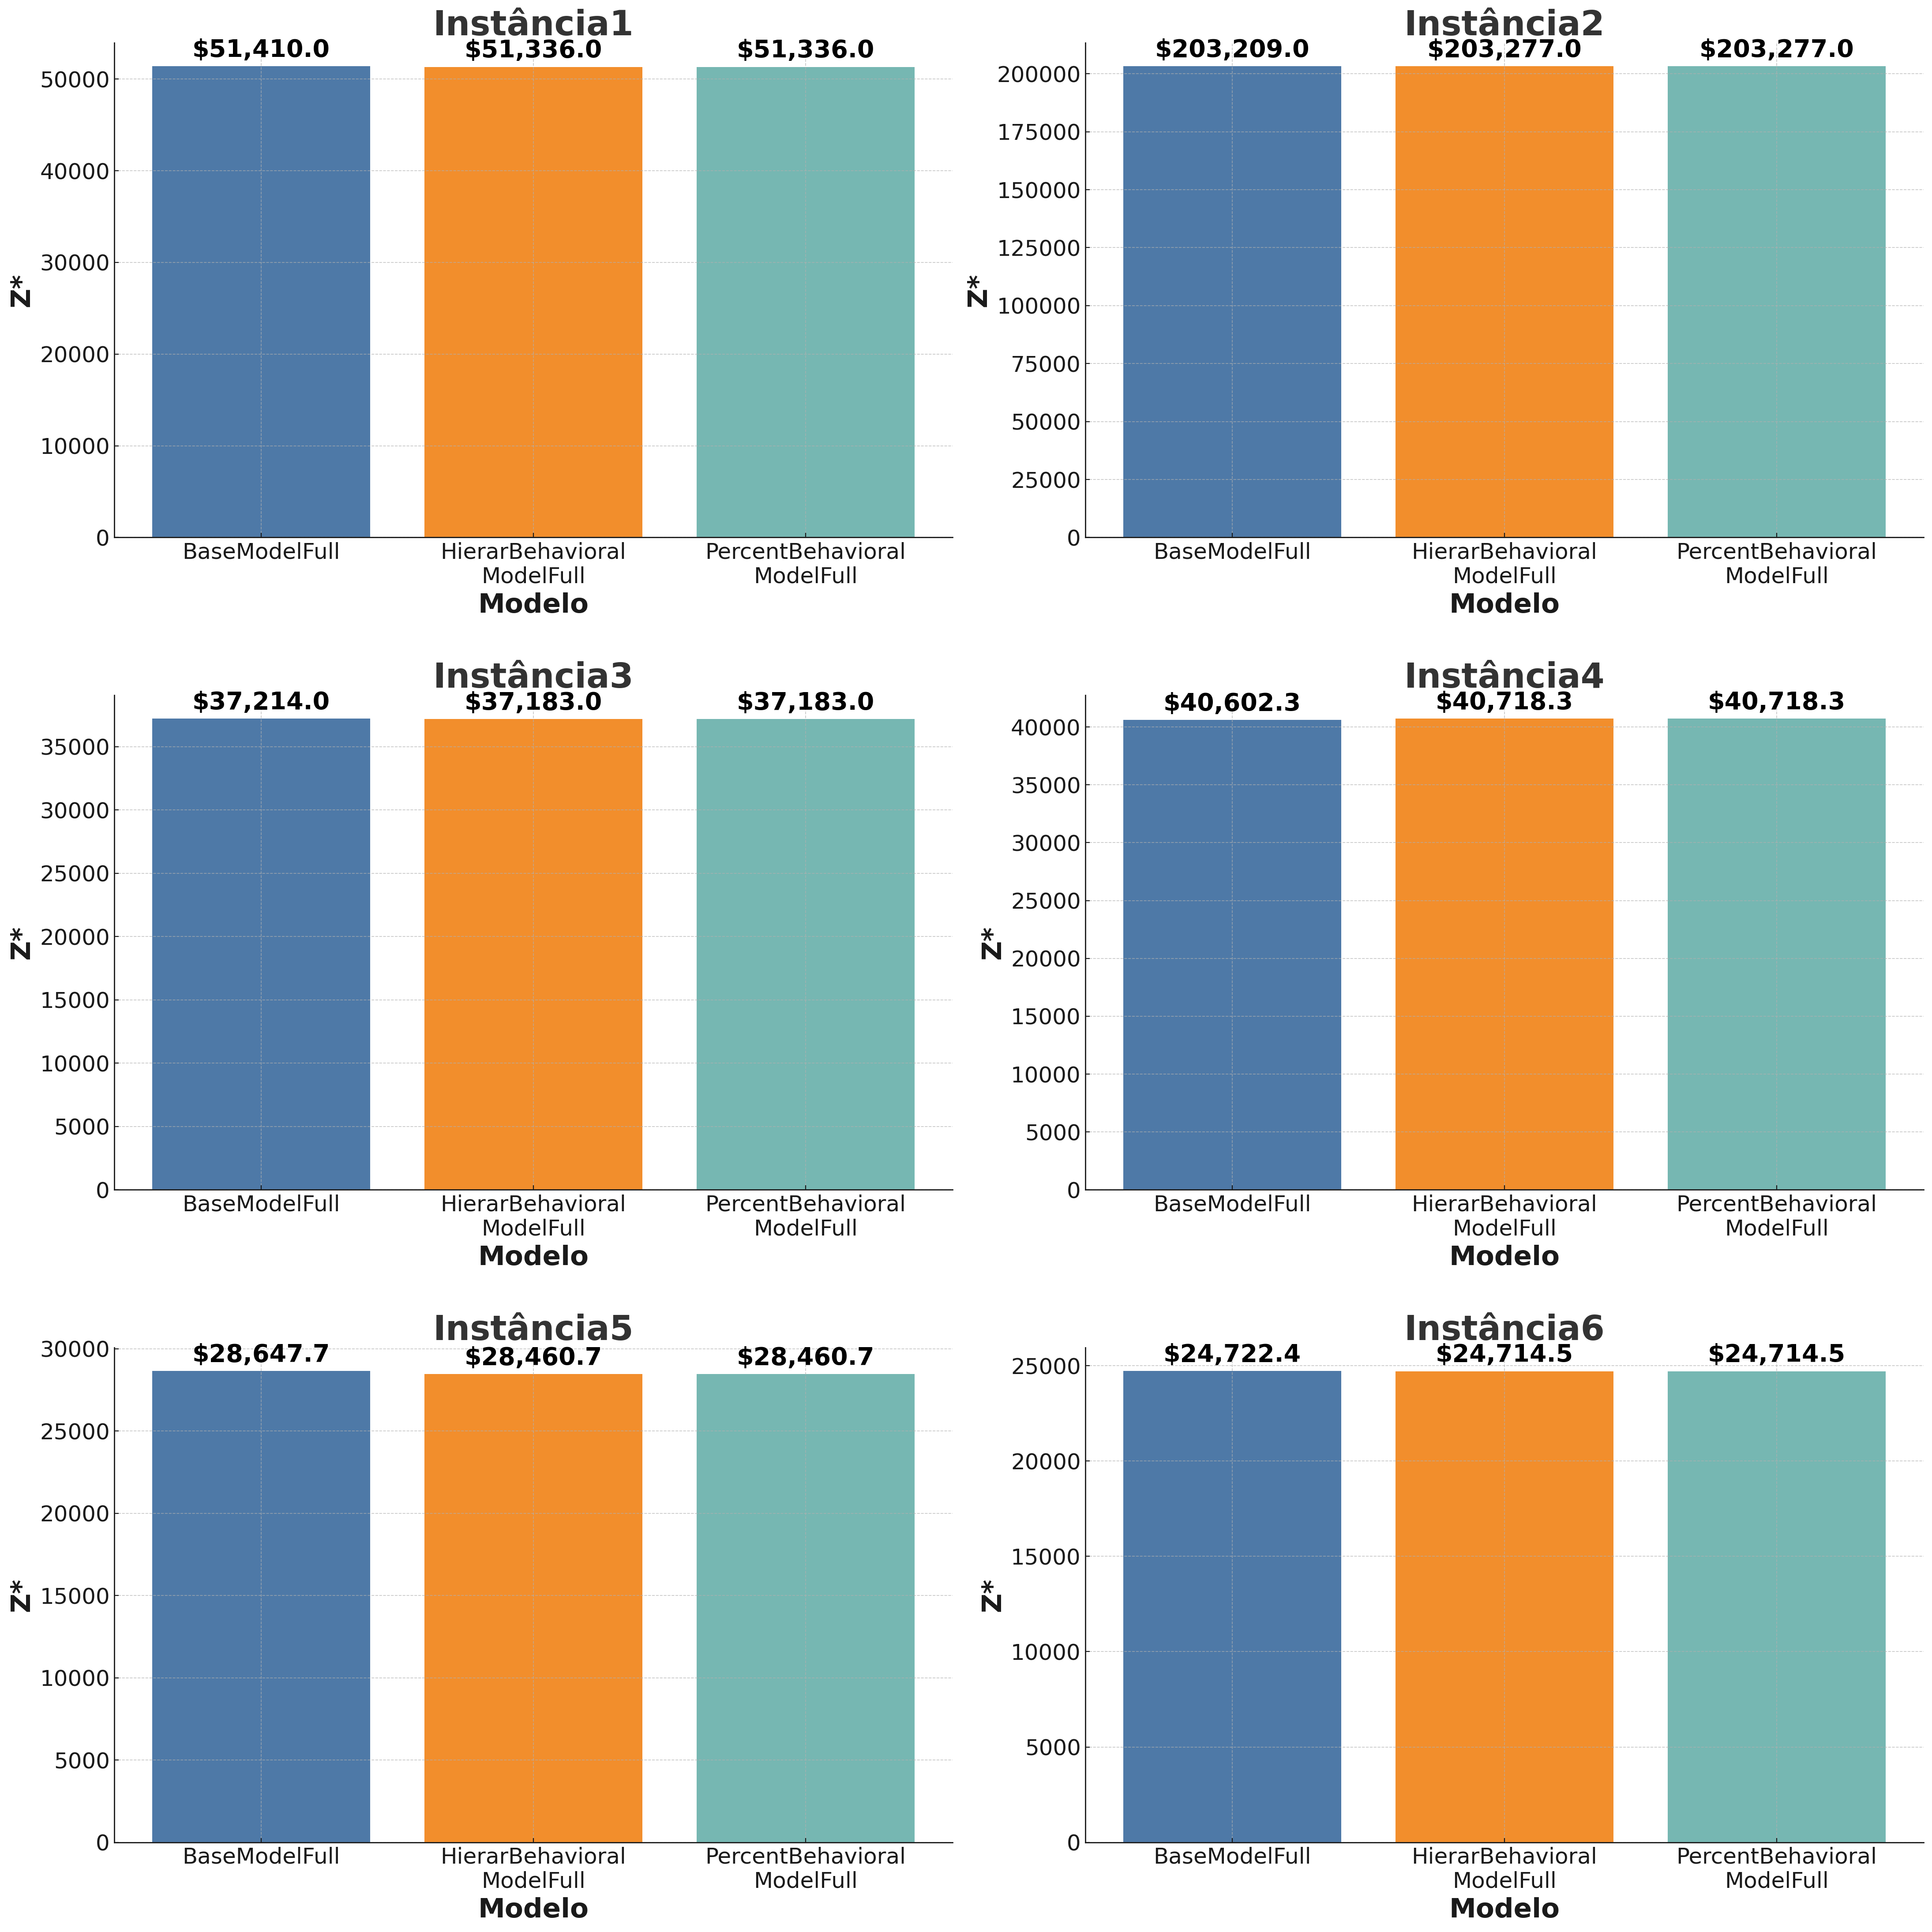
\includegraphics[scale=0.28]{img/compFull1.png}
		\caption{Comparação Modelos Full primeira parte}
		% Fonte:~\cite{khaksar2013genetic}}
		\label{fig: compfull1}
	\end{center}
\end{figure}

\begin{figure}[!ht]
	\begin{center}
		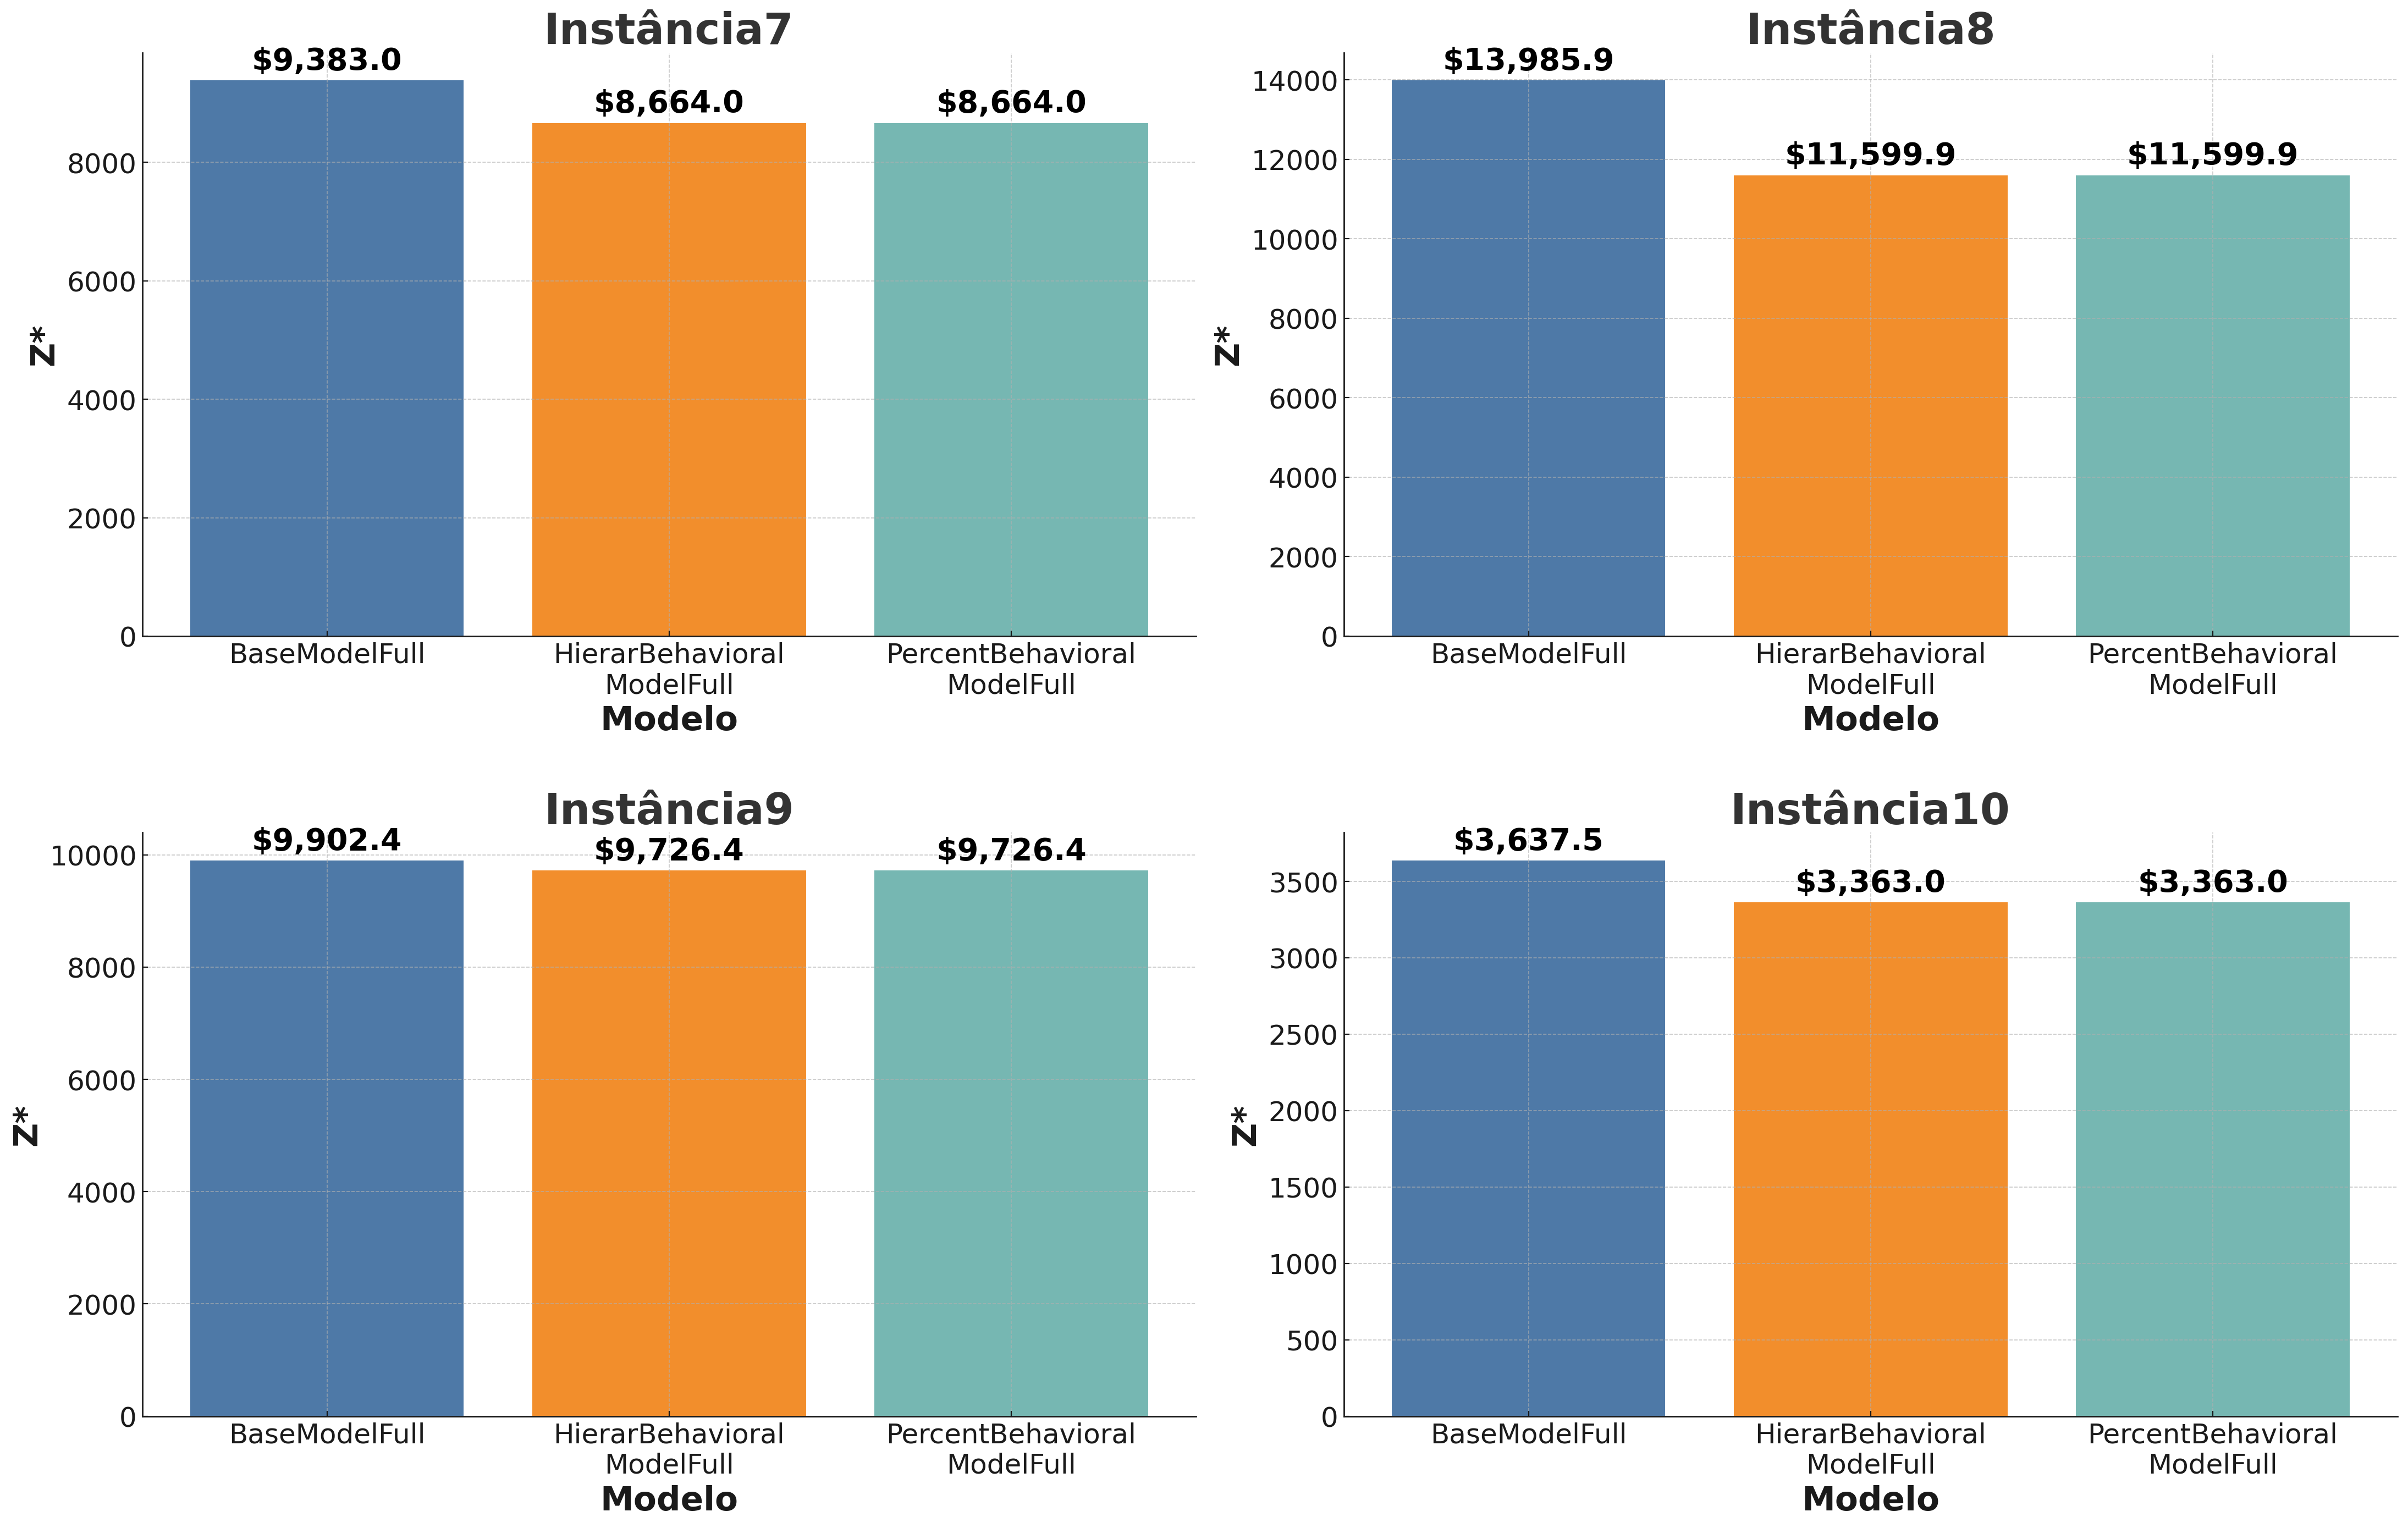
\includegraphics[scale=0.28]{img/compFull2.png}
		\caption{Comparação Modelos Full segunda parte}
		% Fonte:~\cite{khaksar2013genetic}}
		\label{fig: compfull2}
	\end{center}
\end{figure}


Dentro dos resultados observados, diversos comportamentos interessantes foram identificados:

\begin{enumerate}
    \item Tempo de solução:
    O tempo necessário para resolver cada modelo em todas as instâncias foi relativamente baixo. Por exemplo:
    \begin{itemize}
    \item Para as instâncias grandes, os tempos variaram entre 0,04 e 0,12 segundos;
    \item Para as instâncias médias, entre 0,02 e 0,08 segundos;
    \item Para as instâncias pequenas, entre 0,00 e 0,07 segundos.
    \end{itemize}

    \item Exploração de nós:
    Os modelos sempre alcançaram a solução ou soluções ótimas explorando, no máximo, um único nó. Isso demonstra que, na maioria dos casos, a solução ótima coincide com a relaxação linear. Quando isso não ocorre, a diferença máxima relativa é de apenas 0,01\%.
    
    \item Modelos com demanda independente:
    \begin{itemize}
        \item Os modelos BaseModel e BaseModelFulfillments produziram exatamente os mesmos resultados em todas as instâncias analisadas;
        \item O modelo BaseModelSkiplagging, em comparação com o BaseModelFulfillments, apresentou uma redução relativa entre 21,25\% e 56,90\% em todas as instâncias, exceto na instância instância2, onde a redução foi de apenas 3,57\%;
        \item O modelo BaseModelFull mostrou uma redução ainda maior, variando entre 21,25\% e 72,24\%, em comparação com o BaseModelSkiplagging, novamente com exceção da instância instância2, onde a redução foi de 3,57\%.
    \end{itemize}

    \item Modelos com demanda comportamental ajustada por proporções:
    \begin{itemize}
        \item Não foram observadas diferenças entre os modelos BaseModel e BaseModelFulfillments;
        \item Ao contrário do comportamento no modelo independente, o modelo PercentBehavioralModelFulfillments apresentou um aumento relativo entre 0,33\% e 8,6\% nas soluções obtidas, em comparação com o modelo HierarBehavioralModel, exceto nas instâncias instância7, instância8 e instância10, onde o HierarBehavioralModel foi inviável. Acredita-se que essa inviabilidade se deva a alguma inconsistência gerada durante o ajuste da demanda, mas a causa exata ainda não foi determinada;
        \item O modelo PercentBehavioralModelFull mostrou uma redução relativa entre 33\% e 70\%, em comparação com o modelo PercentBehavioralModelSkiplagging.
    \end{itemize}

    \item Modelos com demanda comportamental ajustada por hierarquia:
    \begin{itemize}
        \item Os modelos HierarBehavioralModel e HierarBehavioralModelFulfillments apresentaram os mesmos resultados em todas as instâncias, exceto nas instâncias instância3 e instância6, onde ocorreram reduções de 0,06\% e 0,01\%, respectivamente;
        \item O modelo HierarBehavioralModelSkiplagging apresentou reduções entre 21,8\% e 56,9\%, exceto na instância instância1, onde a redução foi de apenas 3,57\%;
        \item O modelo HierarBehavioralModelFull registrou reduções consideráveis em relação ao modelo HierarBehavioralModelSkiplagging, variando entre 33\% e 74\%.
    \end{itemize}

    \item Análise dos modelos Full (BaseModelFull, HierarBehavioralModelFull, PercentBehavioralModelFull):
    \begin{itemize}
        \item Considerando apenas os modelos Full, ou seja, aqueles que incluem todos os conjuntos de restrições, os modelos comportamentais obtiveram exatamente os mesmos resultados para a função objetivo em cada instância. No entanto, como algumas instâncias possuem múltiplas soluções ótimas, os valores das variáveis de decisão podem diferir, mesmo que os valores da função objetivo sejam iguais;
        \item Além disso, a diferença entre os modelos comportamentais e o modelo independente foi de, no máximo, 2\%, exceto nas instâncias instância7 e instância8, onde as variações foram de 7,7\% e 16,1\%, respectivamente.
    \end{itemize}

\end{enumerate}


Esse detalhamento evidencia o comportamento dos modelos e suas respectivas eficiências em diferentes cenários e ajustes.
% \input{Conclusoes}



% %=============================== Referências Bibliográficas===========================
% \addcontentsline{toc}{chapter}{Bibliografia}\label{referencias}
%\begin{spacing}{0.1}
% \bibliographystyle{agsm,dcu,kluwer, abbrvnat, unsrtnat} choose one
% \bibliographystyle{agsm}
% \bibliography{referencias}
%\end{spacing}
\printbibliography %Prints bibliography
% %=============================== Anexos ==========================
% \appendix
% \renewcommand{\appendixname}{Appendix} %trocar Apendice por Anexo
% \include{G-Appendix}

\end{document}